\documentclass[12pt]{article}
\RequirePackage{amsthm,amsmath,amsbsy,amsfonts}
\usepackage{graphicx}
%\usepackage{enumerate}
\usepackage{natbib}
\usepackage{url} % not crucial - just used below for the URL 
\usepackage{placeins}

%\pdfminorversion=4
% NOTE: To produce blinded version, replace "0" with "1" below.
\newcommand{\blind}{0}

% DON'T change margins - should be 1 inch all around.
\addtolength{\oddsidemargin}{-.5in}%
\addtolength{\evensidemargin}{-.5in}%
\addtolength{\textwidth}{1in}%
\addtolength{\textheight}{1.3in}%
\addtolength{\topmargin}{-.8in}%


\begin{document}
	
	%\bibliographystyle{natbib}
	
	\def\spacingset#1{\renewcommand{\baselinestretch}%
		{#1}\small\normalsize} \spacingset{1}
	
	
	%%%%%%%%%%%%%%%%%%%%%%%%%%%%%%%%%%%%%%%%%%%%%%%%%%%%%%%%%%%%%%%%%%%%%%%%%%%%%%
	
	\if0\blind
	{
		\title{\bf Drift Removal for Time Series Data Using Quantile Trend Filtering}
		\author{Halley Brantley\thanks{
				Department of Statistics, North Carolina State University, Raleigh, NC 27695 (E-mail: hlbrantl@ncsu.edu)} \,
			Joseph Guinness\thanks{
				Department of Biological Statistics and Computational Biology, Cornell University, Ithaca, NY 14853 (E-mail: guinness@cornell.edu )} \,
			and
			%    and
			Eric C. Chi\thanks{Department of Statistics, North Carolina State University, Raleigh, NC 27695 (E-mail: eric$\_$chi@ncsu.edu).}    \\}
		\date{}
		\maketitle
	} \fi
		
	\if1\blind
	{
		\bigskip
		\bigskip
		\bigskip
		\begin{center}
			{\LARGE\bf Title}
		\end{center}
		\medskip
	} \fi
	
	\bigskip
	\begin{abstract}
		The text of your abstract.  200 or fewer words.
	\end{abstract}
	
	\noindent%
	{\it Keywords:}  3 to 6 keywords, that do not appear in the title
	\vfill
	
	\newpage
	\spacingset{1.5} % DON'T change the spacing!
	\section{Introduction}
	\label{sec:intro}
	
	We propose to use the trend filtering penalty with the check loss function to produce a non-parametric quantile regression estimate for removing trends in time series. The formulation was proposed by \cite{Kim2009} as a possible extension of $\ell_1$-trend filtering but not studied. Moreover we extend the basic framework to ensure non-crossing while modeling multiple quantiles. We also implement a parallel ADMM algorithm for series that are too large to be computed simultaneously and proposed a modified criteria for choosing the smoothing parameter. We demonstrate through simulation studies that our proposed model provides better or comparable estimates of non-parametric quantile trends than existing methods and is a more effective method of drift removal for low-cost air quality sensors. 
		
	\subsection{Quantile Regression}
	
	The classic least squares regression is notoriously sensitive to outliers. One remedy to blunt the influence of outliers is to compute the least absolute deviations (LAD) solution in place of the least squares one. Given a design matrix $\mathbf{X} \in \mathbb{R}^{n \times p}$ and continuous responses $y \in \mathbb{R}^n$, we estimate a regression vector $\theta \in \mathbb{R}^p$ so that $\mathbf{X}\theta$ is a good approximation of $y$. The LAD estimator is a solution to the problem
	\begin{eqnarray}
		\underset{\theta}{\min}\; \frac{1}{n}\lVert y - \mathbf{X}\theta \rVert_1.
	\end{eqnarray}
	The above optimization problem generalizes the notion of the median of a collection of numbers. A median $\mu$ of $n$ reals $y_1, \ldots, y_n$ is the minimizer of the function
	\begin{eqnarray}
		f(u) & = & \frac{1}{n}\sum_{i=1}^n \lvert y_i - \theta \rvert.
	\end{eqnarray}
	Recall that the median is the 50th percentile or 0.5-quantile, namely half of the $y_i$ are less than or equal to $\mu$ and the other half is greater than or equal to $\mu$. The median can be generalized to arbitrary $\tau$-quantiles for $\tau \in (0,1)$ to give us quantile regression \citep{Koenker1978}.
	
	First define the so-called "check function"
	\begin{eqnarray}
		\rho_\tau(\Delta) & = & \begin{cases}
			\tau \Delta & \Delta \geq 0 \\
			-(1-\tau)\Delta & \Delta < 0 \\
		\end{cases}
	\end{eqnarray}
	Then the $\tau$th quantile of the $y_i$ is a minimizer of the function
	\begin{eqnarray}
		f_\tau(\theta) & = & \frac{1}{n}\sum_{i=1}^n \rho_\tau(y_i - \theta).
	\end{eqnarray}
	Returning to the regression context, we can generalize LAD regression to quantile regression, namely computing the minimizer of the function
	\begin{eqnarray}
		f_\tau(\theta) & = & \frac{1}{n}\sum_{i=1}^n \rho_\tau(y_i - \langle x_i \mid \theta \rangle),
	\end{eqnarray}
	where $x_i \in \mathbb{R}^p$ denotes the $i$th row of $\mathbf{X}$.
	
	%% ----------------------------------------------------------------------
	%% Trend Filtering
	%% ----------------------------------------------------------------------
	\subsection{Trend Filtering}
	
	In the trend filtering problem \citep{Kim2009, Tib2014}, one is interested in finding an adaptive polynomial approximation to noisy data $y \in \mathbb{R}^n$ by solving the following convex problem.
	\begin{eqnarray}
		\underset{\theta}{\arg\min}\; \frac{1}{2n} \lVert y - \theta \rVert_2^2 + \lambda \lVert \mathbf{D}^{(k+1)}\theta \rVert_1,
	\end{eqnarray}
	where $\lambda \geq 0$ is a regularization parameter that trades off the emphasis on the data fidelity term and the matrix $\mathbf{D}^{(k+1)} \in \mathbb{R}^{(n - k -1) \times n}$ is the discrete difference operator of order $k+1$. To understand the purpose of penalizing $\mathbf{D}^{(k+1)}$ consider the difference operator when $k = 0$.
	\begin{eqnarray}
		\mathbf{D}^{(1)} = \begin{pmatrix}
			-1 & 1 & 0 & \cdots & 0 & 0 \\
			0 & -1 & 1 & \cdots & 0 & 0 \\
			\vdots & & & & & \\
			0 & 0 & 0 & \cdots & -1 & 1 \\
		\end{pmatrix}
	\end{eqnarray}
	Thus, $\lVert \mathbf{D}^{(1)}\theta \rVert_1 = \sum_{i=1}^{n-1} \lvert \theta_i - \theta_{i+1} \rvert$ which is just total variation denoising in one dimension. The penalty incentivizes solutions which are piece-wise constant. For $k \geq 1$, the difference operator $\mathbf{D}^{(k+1)} \in \mathbb{R}^{(n-k-1) \times n}$ is defined recursively as follows
	\begin{eqnarray}
		\mathbf{D}^{(k+1)} & = & \mathbf{D}^{(1)}\mathbf{D}^{(k)}.
	\end{eqnarray}
	By penalizing the $k+1$ fold composition of the discrete difference operator, we obtain solutions which are piecewise polynomials of order $k$.
	
	%% ----------------------------------------------------------------------
	%% Quantile Trend Filtering
	%% ----------------------------------------------------------------------
	\section{Methods}
	
	\subsection{Quantile Trend Filtering}
	
	We combine the ideas of quantile regression and trend filtering, namely consider the signal approximation problem, where the design $\mathbf{X}$ is the identity matrix.
	
	The estimation of the quantile trend filtering model can be posed as the following optimization problem.
	\begin{eqnarray}
	\label{eq:quantile_trend}
	\underset{\theta}{\min}\; \frac{1}{n} \sum_{i=1}^n \rho_\tau(y_i - \theta_i) + \lambda \lVert \mathbf{D}^{(k)} \theta \rVert_1,
	\end{eqnarray}
	where $\lambda$ is a non-negative tuning parameter. As with the classic quantile regression, the quantile trend filtering problem can be solved by a linear program. 
	
	\subsection{Smoothing parameter choice}
	Our method can easily handle missing data by changing the check loss function to output 0 for missing values. This allows us to leave out validation observations that can be used to select the tuning parameter $\lambda$ and to compare method performance on real data. A number of methods have been proposed for selecting the quantile regression smoothing spline tuning parameter \cite{yuan2006gacv}.  \cite{KoenkerNgPortnoy1994} relate $\lambda$ to the number of interpolated points $p_{\lambda} = \sum I(y_i = \widehat{g}_i(x_i))$, which can be thought of as active knots, they propose the Schwarz criterion for the selection of $\lambda$
	\begin{equation}
	SIC(p_{\lambda}) = log[n^{-1}\sum\rho_{\tau}(y_i - \widehat{g}(x_i))] + \frac{1}{2n}p_{\lambda}log n
	\end{equation}
	
	The traditional Bayesian Information Criterion (BIC) is given by 
	\begin{equation}
	\mbox{BIC}(s) = -2\log(L\{\hat{\theta}(s)\}) + \nu(s)\log n 
	\end{equation}	
	where $\theta(s)$ is the parameter $\theta$ with those components outside $s$ being set to 0, and $\nu(s)$ is the number of components in $s$. If we assume an asymmetric Laplace likelihood $L(y|\theta) = \left(\frac{\tau^n(1-\tau)}{\sigma}\right)^n\exp\left\{-\sum_i\rho_\tau(\frac{y_i - \theta_i}{\sigma})\right\}$ and the number of non-zero elements of $D\theta$ as $df$
	\begin{equation}
	\mbox{BIC}(df) = 2\sum_i\frac{1}{\sigma}\rho_{\tau}(y_i-\theta_i) + df\log n
	\end{equation} 
	We can choose and $\sigma>0$ and have found empirically that $\sigma =  \frac{1-|1-2\tau|}{2}$ produces stable estimates. \cite{chen2008} proposed the extended BIC for large parameter spaces 
	\begin{equation}
	BIC_{\gamma}(s) = -2\log(L\{\hat{\theta}(s)\}) + \nu(s)\log n  + 2\gamma\log{P\choose j,}~~\gamma \in [0,1]
	\end{equation}
	where $P$ is the total number of possible parameters and $j$ is the number of parameters included in given model. We used this criteria with $\gamma = 1$, $P=n-k$ where $k$ is the order of the differencing matrix and $j = \nu(s)$ is the number of non-zero entries in $D^{(k)}\theta$. 

	We used a single dataset to illustrate the difference between the scaled, unscaled and extended BIC criteria. 
	
	\begin{figure}[h!]
	\caption{Degrees of freedom (number of non-zero elements of $D\theta$) by $\log(\lambda)$.} 
	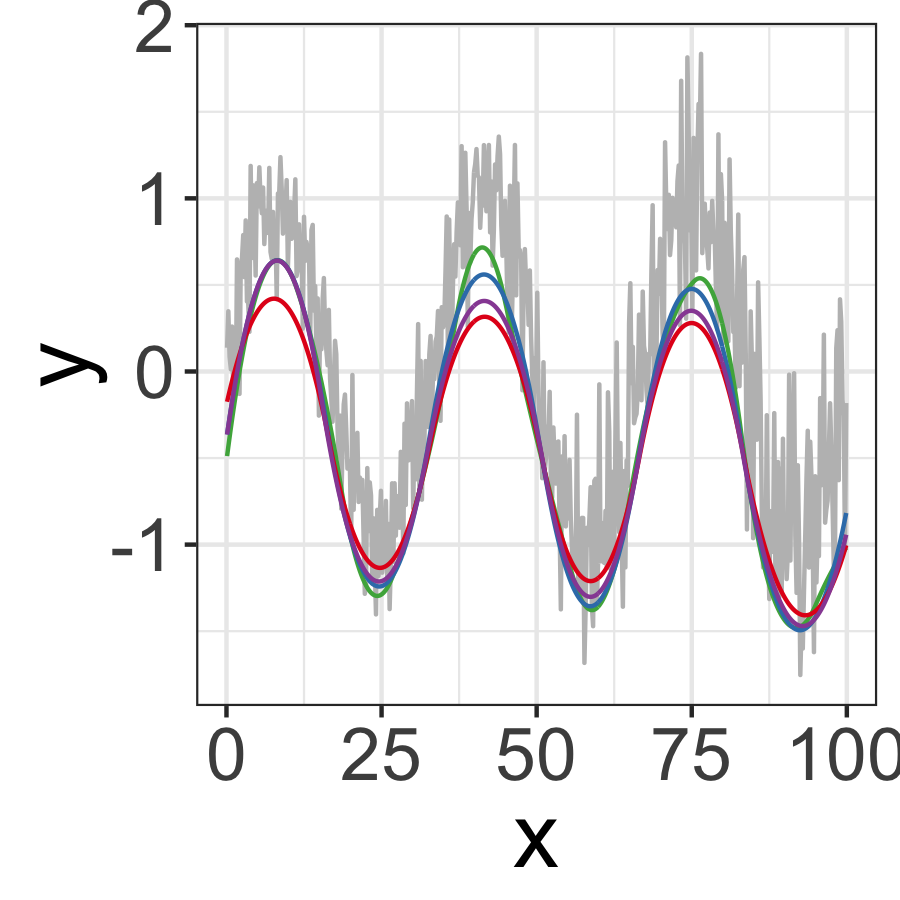
\includegraphics[width = 0.25\linewidth]{Figures/BIC_data.png}
	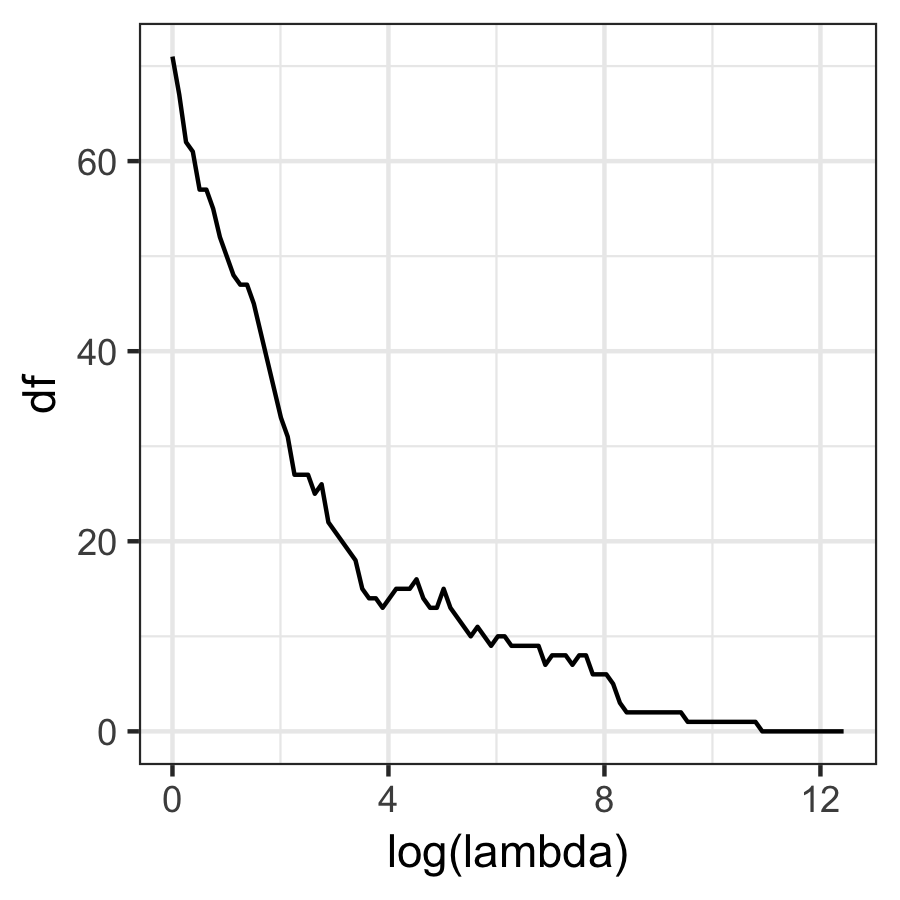
\includegraphics[width = 0.25\linewidth]{Figures/df_by_lambda.png}
	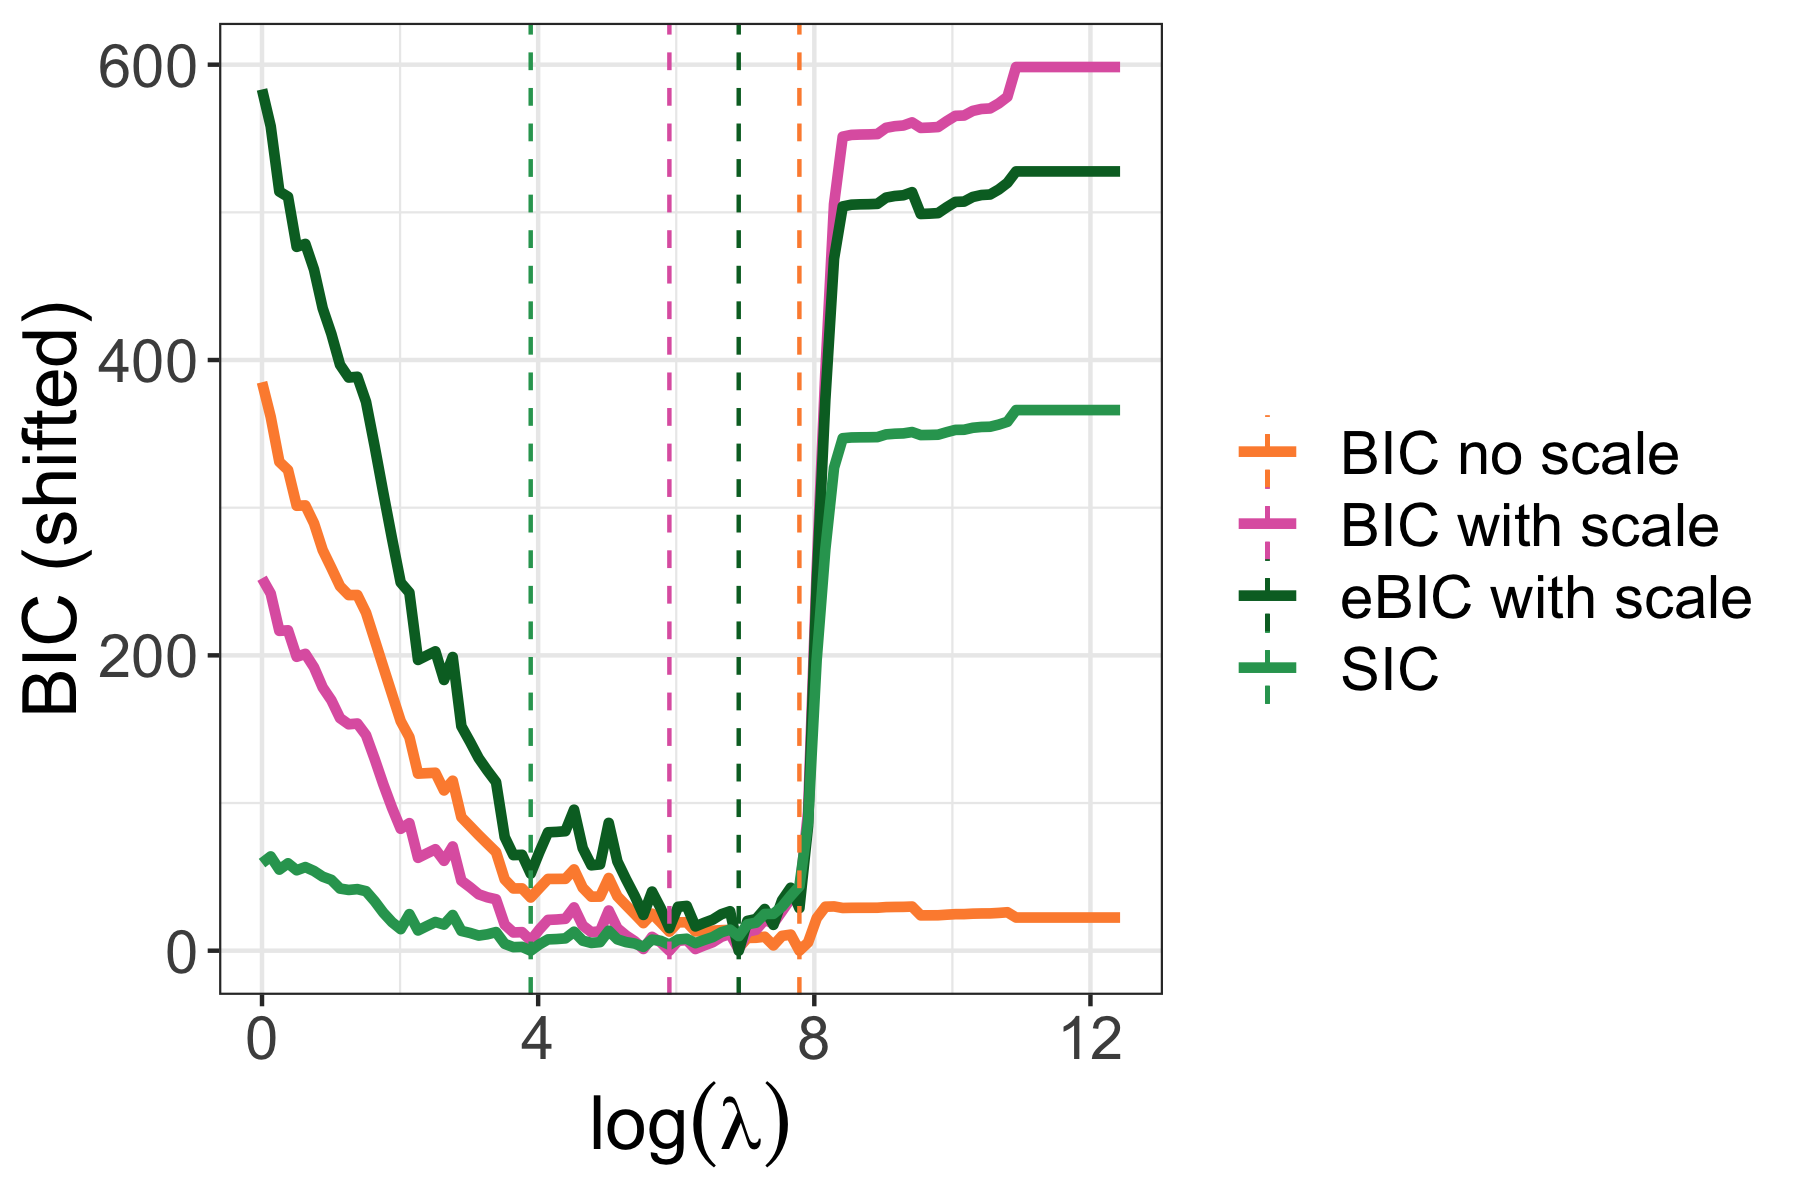
\includegraphics[width = 0.5\linewidth]{Figures/BIC_by_lambda.png}
	\end{figure}

	\subsection{ADMM for Smoothing Windows}
	
	To our knowledge, no one has addressed the problem of finding smooth quantile trends of series that are too large to be processed simultaneously. We propose an alternating direction method of multipliers (ADMM) algorithm for solving large problems in a piecewise fashion. The ADMM algorithm, described by \cite{boyd2011distributed}, relies on the idea of dual ascent. If we consider the equality optimization problem 
	\begin{align}
	&\text{minimize } f(x)\\
	&\text{subject to } Ax = b
	\end{align}
	with variable $x\in \mathbf{R}^n$, where $A \in \mathbf{R}^{mxn}$ and $f: \mathbf{R}^n \rightarrow \mathbf{R}$ is convex. The corresponding Lagrangian function is 
	\begin{equation}
	L(x,\omega) = f(x) + \omega^T(Ax-b)
	\end{equation}
	and the corresponding dual problem  is 
	\begin{equation}
	\text{maximize } \inf_x L(x,\omega)
	\end{equation}
	Assuming that strong duality holds (Slater's constraint: there exists a solution in the interior of the domain), the optimal values of the primal and dual variables are the same. The dual ascent method, uses gradient ascent to solve the dual problem and thus the primal problem using the iterates
	\begin{align}
	&x^{k+1} = \arg\min L(x, \omega^k)\\
	&\omega^{k+1} = \omega^k + \alpha^k(Ax^{k+1} - b)
	\end{align}
	where $\alpha^k > 0$ is a step size and $k$ is the iteration counter. In many cases (including our problem), the $x$ update fails because the problem is unbounded below. To remedy this issue the augmented Lagrangian was introduced:
	\begin{equation}
	L_{\gamma}(x,\omega) = f(x)+\omega^T(Ax-b) + \frac{\gamma}{2}||Ax-b||_2^2
	\end{equation}
	where $\gamma > 0$ is called the penalty parameter. Applying dual ascent to the modified problem results in the method of multipliers algorithm which converges under more general conditions:
	\begin{align}
	&x^{k+1} = \arg\min L_\gamma(x, \omega^k)\\
	&\omega^{k+1} = \omega^k + \gamma(Ax^{k+1} - b)
	\end{align}
	Consider a new optimization problem with a separable objective function. 
	\begin{align}
	&\text{minimize } f_1(x_1) + f_2(x_2)\\
	&\text{subject to } A_1x_1 + A_2x_2 = b
	\end{align}
	where $x = (x_1, x_2)$, $i \in \{1,2\}$, and  $x_i \in \mathbf{R}^{n_i}$. The dual ascent updates can be expressed as 
	\begin{align}
	&x_i^{k+1} = \arg\min L_i(x_i, \omega^k)\\
	&\omega^{k+1} = \omega^k + \alpha^k(Ax^{k+1} - b)
	\end{align}
	however we lose the separability if the augmented Lagrangian is used instead, i.e. the augmented Lagrangian can not be separated into functions of $x_i$.  The Alternating Direction Method of Multipliers (ADMM) addresses this problem and maintains separability while using the augmented Lagrangian to improve convergence through the following updates
	\begin{align}
	&x_1^{k+1} = \arg\min_{x_1} L_{\gamma}(x_1, x_2^k, \omega^k)\\
	&x_2^{k+1} = \arg\min_{x_2} L_{\gamma}(x_1^{k+1}, x_2, \omega^k)\\
	&\omega^{k+1} = \omega^k + \alpha^k(A_1x_1^{k+1} + A_2x_2^{k+1} - b)
	\end{align}
	
	We now consider the quantile regression trend filtering problem,  
	\begin{equation}
	\text{minimize } \rho_\tau(y-\theta) + \lambda||D^{(k)}\theta||_1\\
	\end{equation}
	where $y,\theta \in \mathbf{R}^n$, $y$ is the observed data, $\rho_{\tau}(u) = \sum_i(\tau - I(u_i < 0))u_i$ is the check loss function corresponding to quantile level $\tau$ and $D^{(k)}$ is the discrete differencing matrix of order $k$ and $\lambda$ is a tuning parameter that controls smoothness. We first re-parameterize $\phi = y-\theta$ so the problem is
	\begin{equation}
	\text{minimize } \rho_\tau(\phi) + \lambda||D^{(k)}(y-\phi)||_1\\
	\end{equation}
	We further divide $\phi$ order to solve smaller problems: Defining
	\begin{align}
	&\phi_1 = (\phi_{11}, \phi_{12})\\
	&\phi_2 = (\phi_{21}, \phi_{22}, \phi_{23})\\
	&\phi_3 = (\phi_{31}, \phi_{32})\\
	&\phi = (\phi_{11}, \phi_{12}=\phi_{21}, \phi_{22}, \phi_{23}=\phi_{31}, \phi_{32}) \\
	\end{align}
	Dividing $y$ similarly, the problem then becomes 
	\begin{align}
	&\text{minimize } \sum_{i=1}^3 \rho_\tau(\phi_i) + \lambda||D^{(k)}(y_i-\phi_i)||_1\\
	&\text{subject to: } \phi_{12}=\phi_{21}, ~~ \phi_{23}=\phi_{31}\\
	\end{align}
	We can further simplify by defining 
	\begin{align}
	&\overline{\phi} = (\phi_{11}, \frac{\phi_{12}+\phi_{21}}{2}, \phi_{22}, \frac{\phi_{23}+\phi_{31}}{2}, \phi_{32}) \\
	&\overline{\phi_1} = (\phi_{11}, \frac{\phi_{12}+\phi_{21}}{2})\\
	&\overline{\phi_2} = ( \frac{\phi_{12}+\phi_{21}}{2}, \phi_{22}, \frac{\phi_{23}+\phi_{31}}{2})\\
	&\overline{\phi_3} = (\frac{\phi_{23}+\phi_{31}}{2}, \phi_{32})
	\end{align}
	so the problem becomes
	\begin{align}
	&\text{minimize } \sum_{i=1}^3 \rho_\tau(\phi_i) + \lambda||D^{(k)}(y_i-\phi_i)||_1\\
	&\text{subject to: } \phi_{i}=\overline{\phi_i}\\
	\end{align}
	The augmented Lagrangian for this problem is 
	\begin{align}
	&L_\gamma(\phi_1,\phi_2, \phi_3, \overline{\phi_1}, \overline{\phi_2}, \overline{\phi_3}, \omega) = \\
	&\sum_{i=1}^3 \rho_\tau(\phi_i) + \lambda||D^{(k)}(y_i-\phi_i)||_1 + \omega_i^T(\phi_i - \overline{\phi_i}) + \frac{\gamma}{2}||\phi_i - \overline{\phi_i}||_2^2
	\end{align}
	The ADMM updates are then given by
	\begin{align}
	&\phi_i^{k+1} = \arg\min_{\phi_i}\rho_\tau(\phi_i) + \lambda||D^{(k)}(y_i-\phi_i)||_1 + \omega_i^{kT}(\phi_i - \overline{\phi_i}^k) + \frac{\gamma}{2}||\phi_i - \overline{\phi_i}^k||_2^2\\
	&\omega_i^{k+1} = \omega_i^{k} + \gamma(\phi_i^{k+1} - \overline{\phi_i}^{k+1})
	\end{align}
	The $\phi_i$ updates can be obtained using a quadratic program solver such as Gurobi and can be obtained in parallel. 
	
	\pagebreak 
	
	\begin{figure}[!h] 
		\caption{Windows fit separately compared to simultaneous fit, no signal present.}
		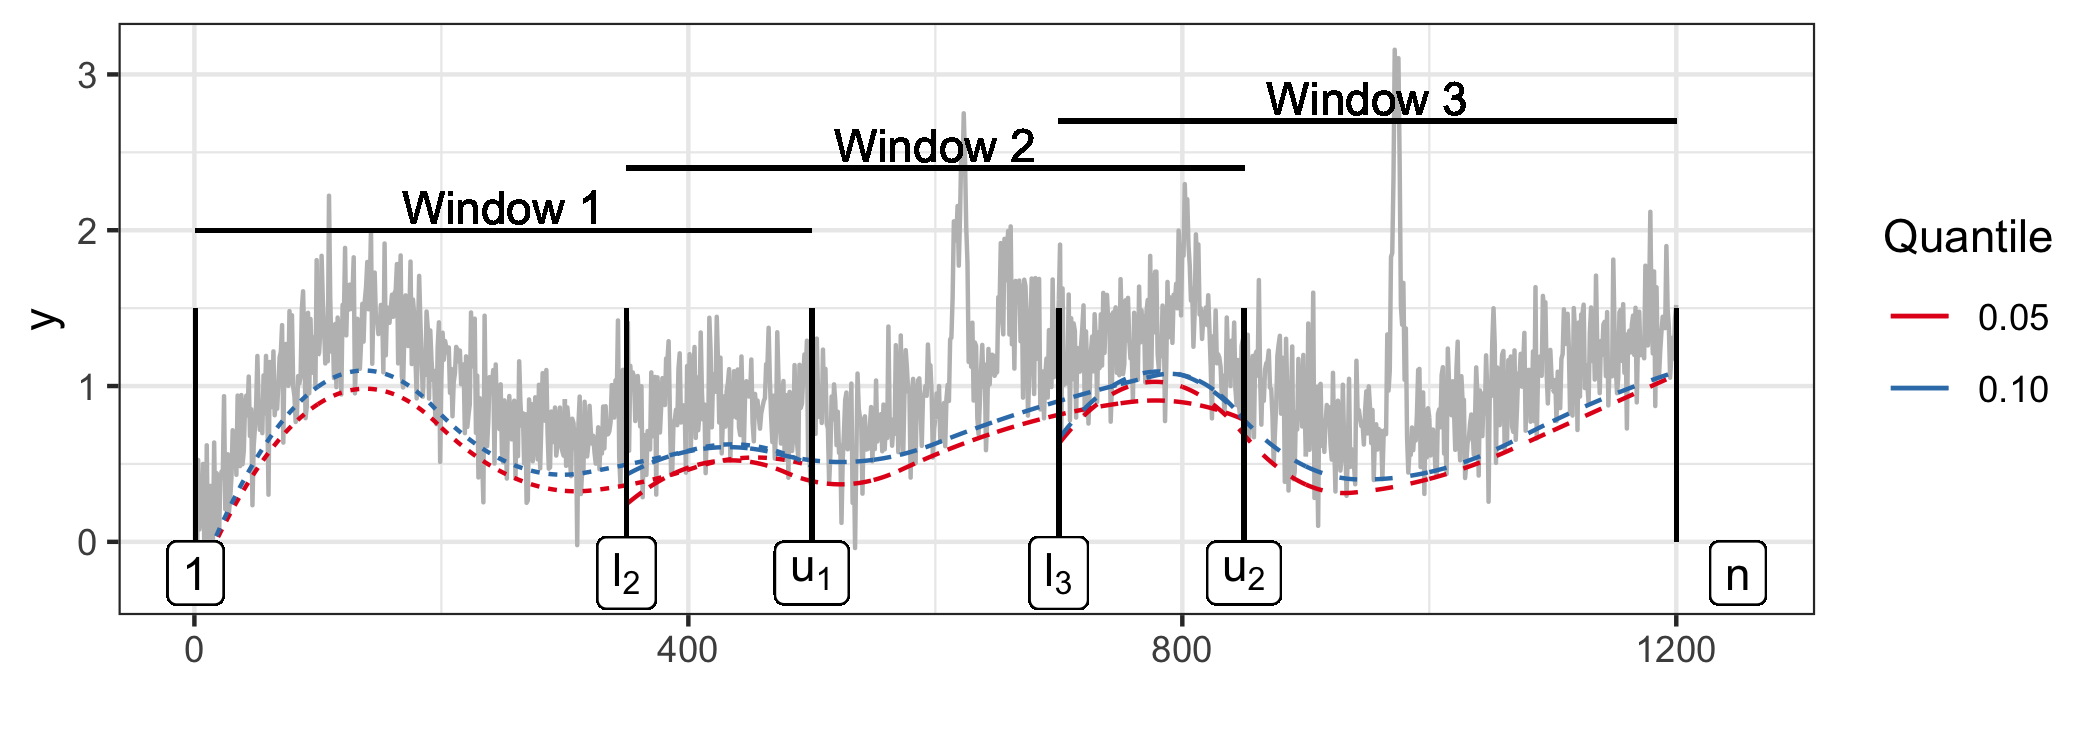
\includegraphics[width = \linewidth]{Figures/overlapping_windows.png}
	\end{figure}
	
	\begin{figure}[!h] 
		\caption{Windows fit with 150 iterations of ADMM, no signal present.}
		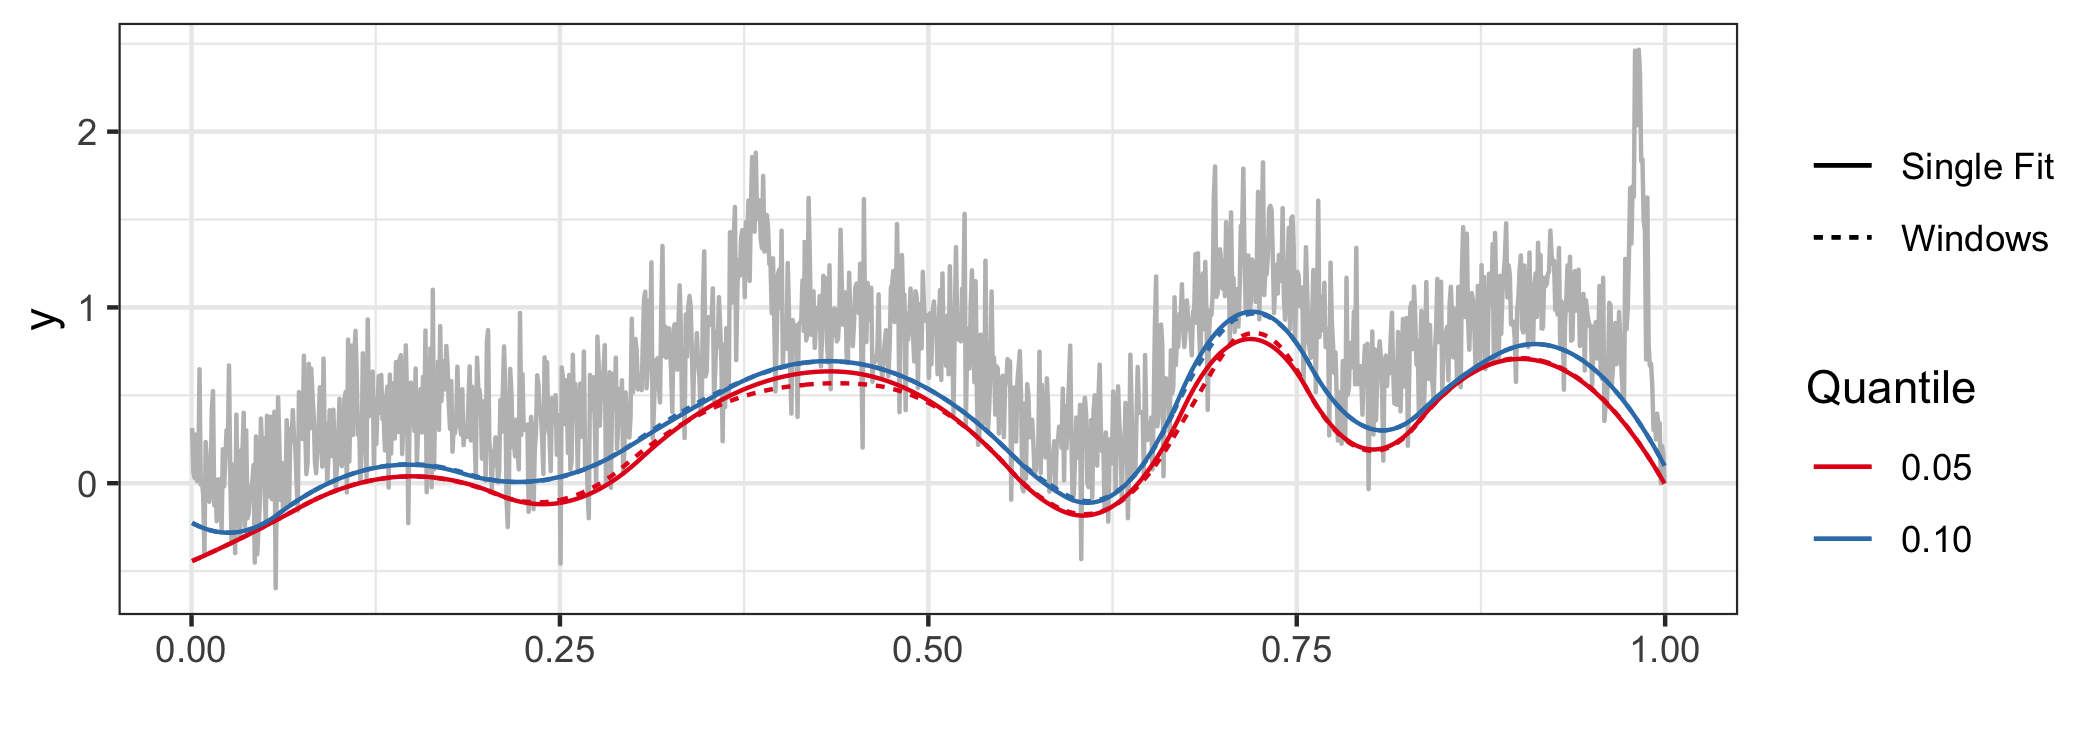
\includegraphics[width = \linewidth]{Figures/admm_windows.png}
	\end{figure}
	
	\begin{figure}[!h] 
		\caption{Windows fit separately compared to simultaneous fit, signal present.}
		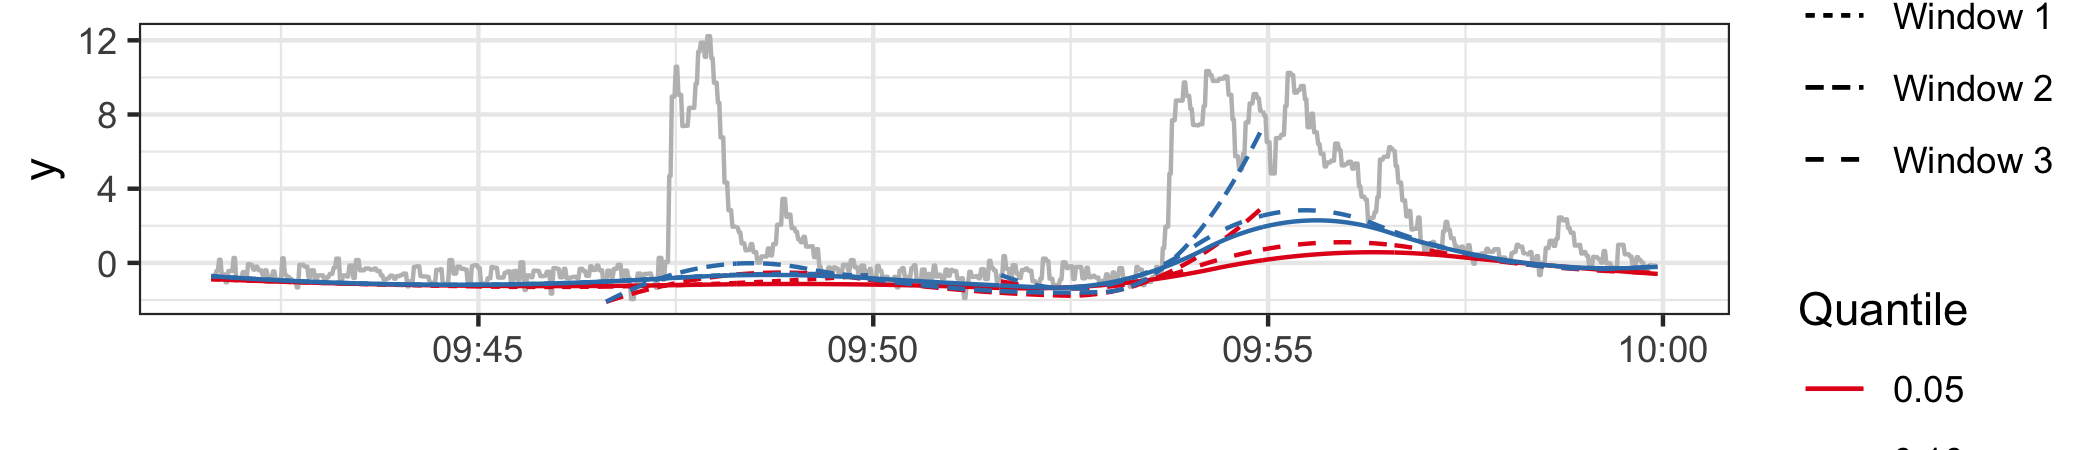
\includegraphics[width = \linewidth]{Figures/overlapping_windows2.png}
	\end{figure}
	
	\begin{figure}[!h] 
		\caption{Windows fit with 300 iterations of ADMM, signal present.}
		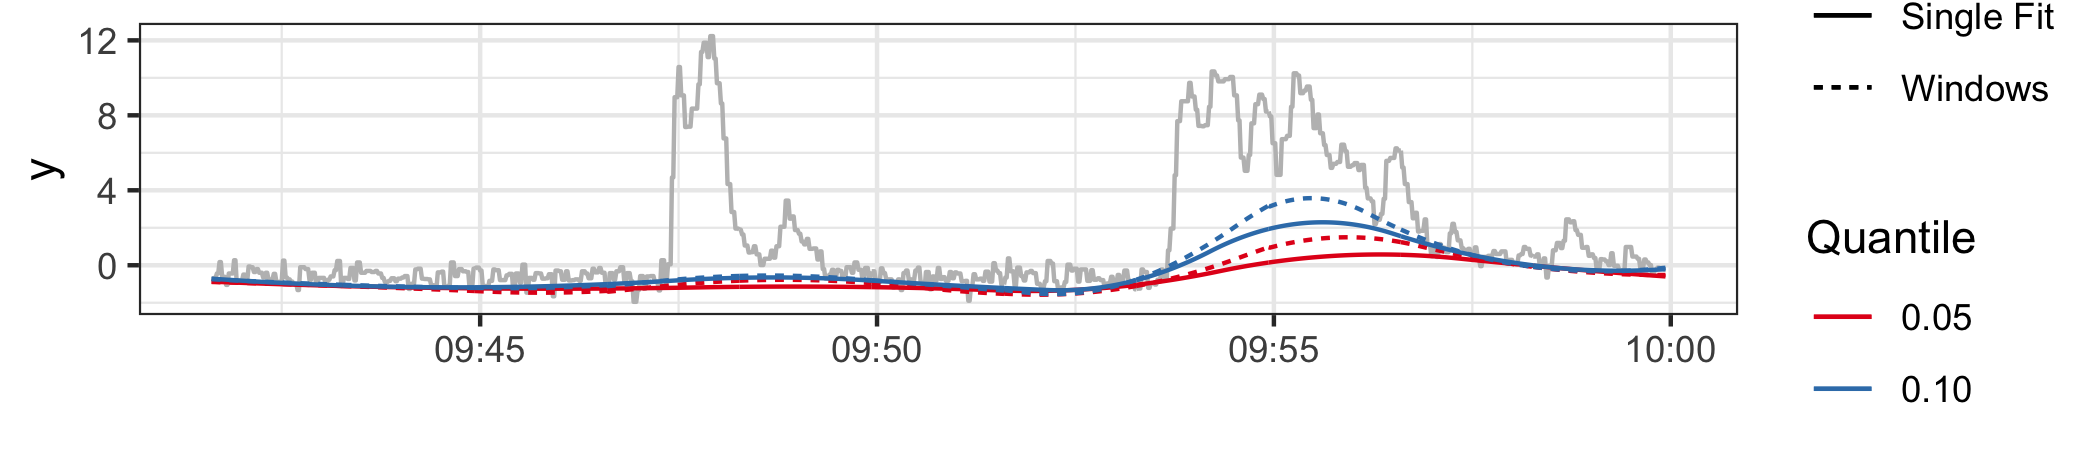
\includegraphics[width = \linewidth]{Figures/admm_windows2.png}
	\end{figure}

	\section{Simulation Study}
	
	We compare the performance of our quantile trend filtering method with the three previously published methods using designs proposed by \cite{Racine2017}. The methods compared are: \texttt{npqw} which is the quantile-ll method described in \cite{Racine2017}, code was obtained from the author; \texttt{qsreg} in the \texttt{fields} R package and described in \cite{Oh2011}; \texttt{rqss} available in the \texttt{quantreg} package and described in \cite{KoenkerNgPortnoy1994}.  The smoothing parameter $\lambda$ for the \texttt{rqss} method is chosen using a grid search and minimizing the SIC criteria as described in \cite{KoenkerNgPortnoy1994}. We further compare three criteria for choosing the smoothing parameter for our detrend method: \texttt{detrendr\_SIC}: Our method where we minimize $\sum_i\rho_{\tau}(y_i - \theta_i) + \lambda||D\theta||_1$ and $\lambda$ is chosen using SIC \citep{KoenkerNgPortnoy1994}.  \texttt{detrendr\_valid}: Our method where lambda is chosen by leaving out every 5th observation as a validation data set and minimizing the evaluating the check loss function evaluated at the validation data. \texttt{detrendr\_eBIC}:  the new criteria we have proposed based on the extended BIC proposed by \cite{chen2008}. 
	 
	Three simulation designs from \cite{Racine2017} were considered. For all designs $X_i$ was generated as a uniformly spaced sequence in $[0,1]$ and the response $Y$ was generated as 
	$$Y_i = sin(2\pi x_i) + \epsilon_i(x_i)$$
	The three error distributions considered were 
	\begin{itemize}
		\item Gaussian: $\epsilon_i(x_i) \sim N\left(0, \left(\frac{1+x_i^2}{4}\right)^2\right)$
		\item Beta: $\epsilon_i \sim Beta(1, 11-10x_i)$
		\item Mixed normal: $\epsilon_i$ is simulated from a mixture of $N(-1,1)$ and  $N(1,1)$ with mixing probability $x_i$.
	\end{itemize}
	\begin{figure}
		\caption{Simulated data with true quantiles $\tau \in \{0.01, 0.05, 0.25, 0.5, .75, 0.95, 0.99\}$}	
		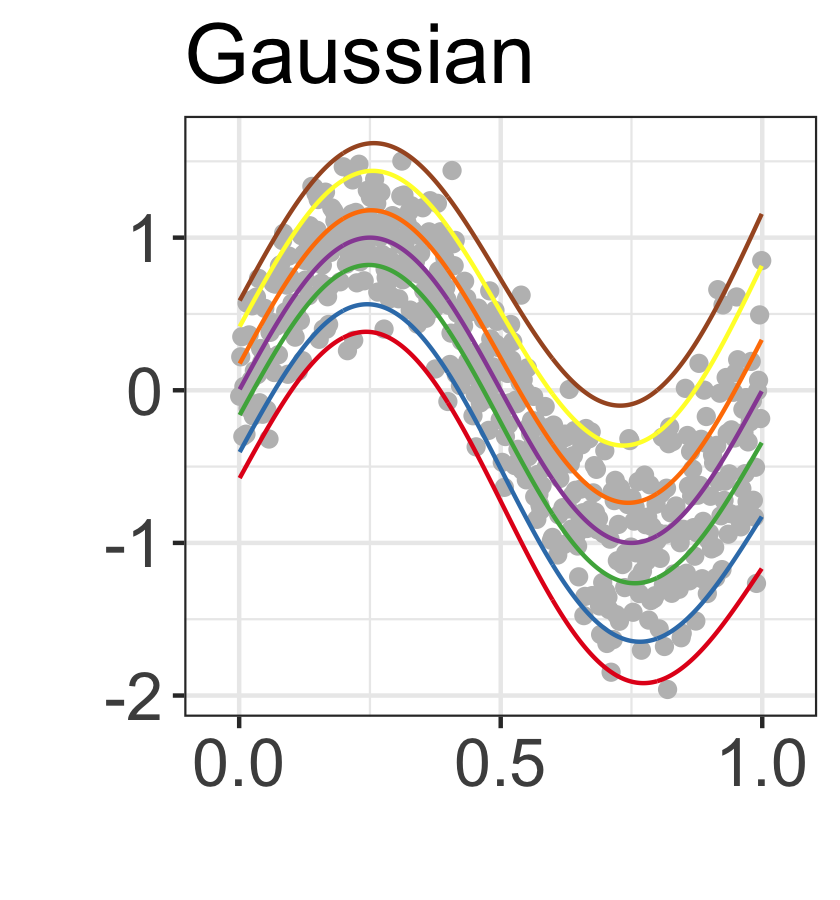
\includegraphics[width=.3\linewidth]{Figures/gaus.png}
		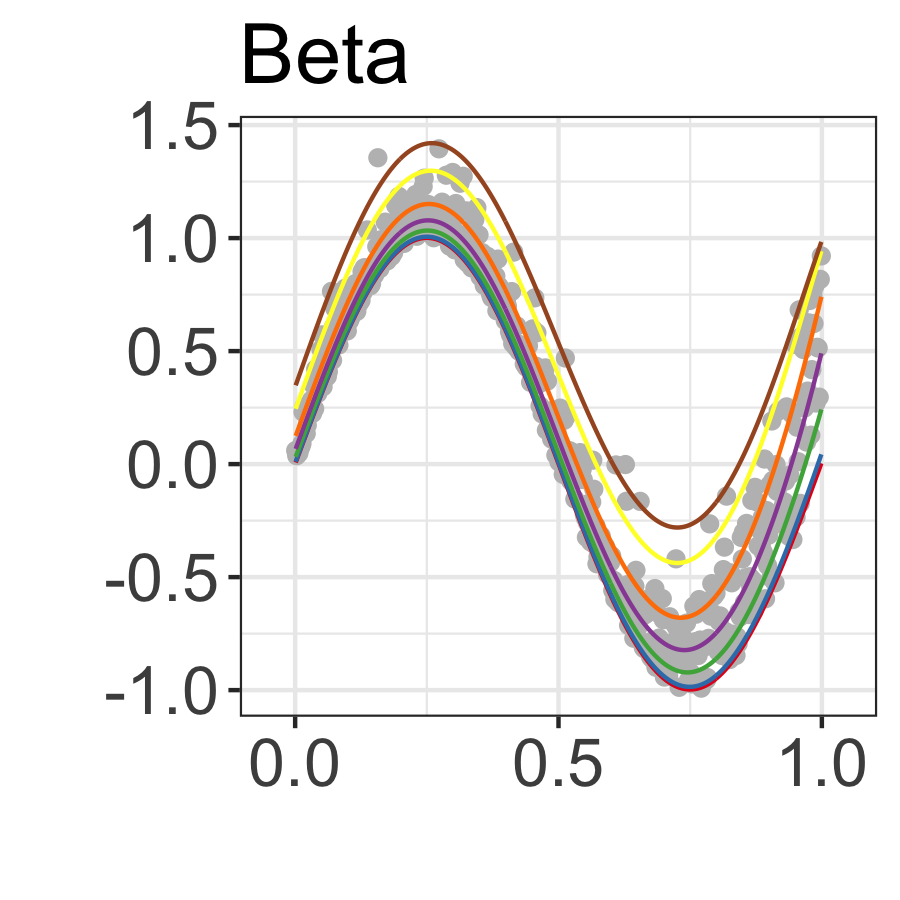
\includegraphics[width=.3\linewidth]{Figures/shapebeta.png}
		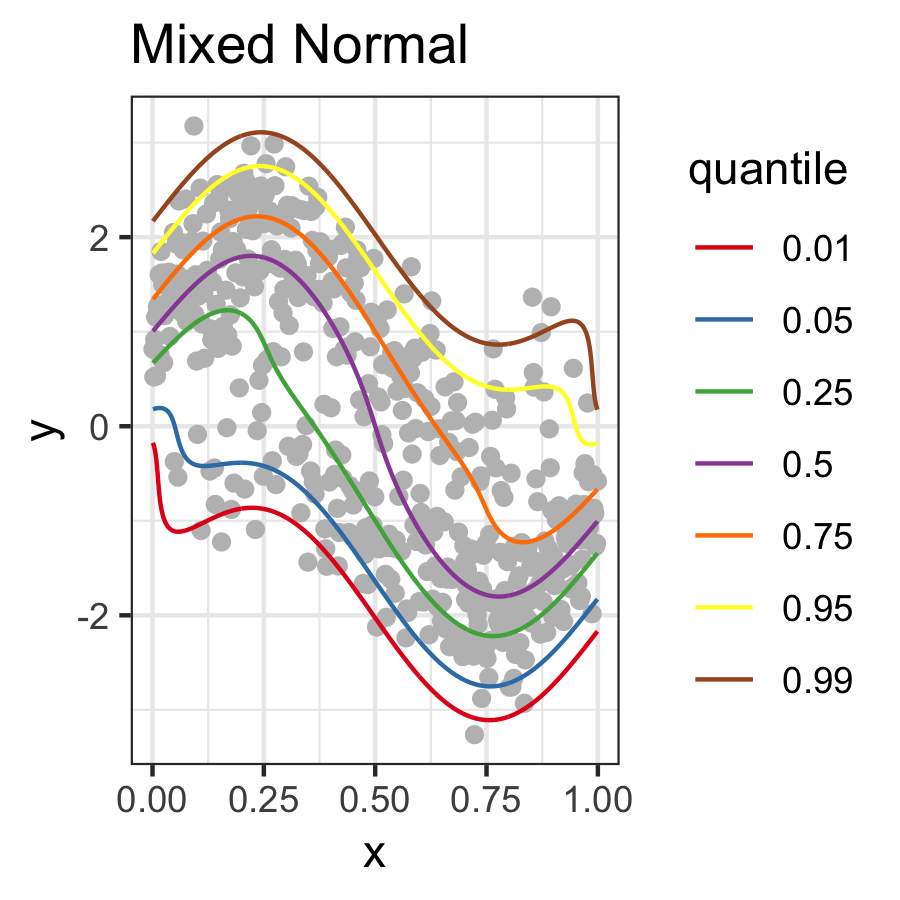
\includegraphics[width=.3\linewidth]{Figures/mixednorm.png}
	\end{figure}
	
	100 datasets were generated of sizes 300, 500 and 1000. The MSE was calculated as $\frac{1}{n}\sum_i (\hat{q}_{\tau}(x_i) - q_\tau(x_i))^2$. The plots below show the mean MSE $\pm$ twice the standard error by method, quantile level and sample size. 
	
	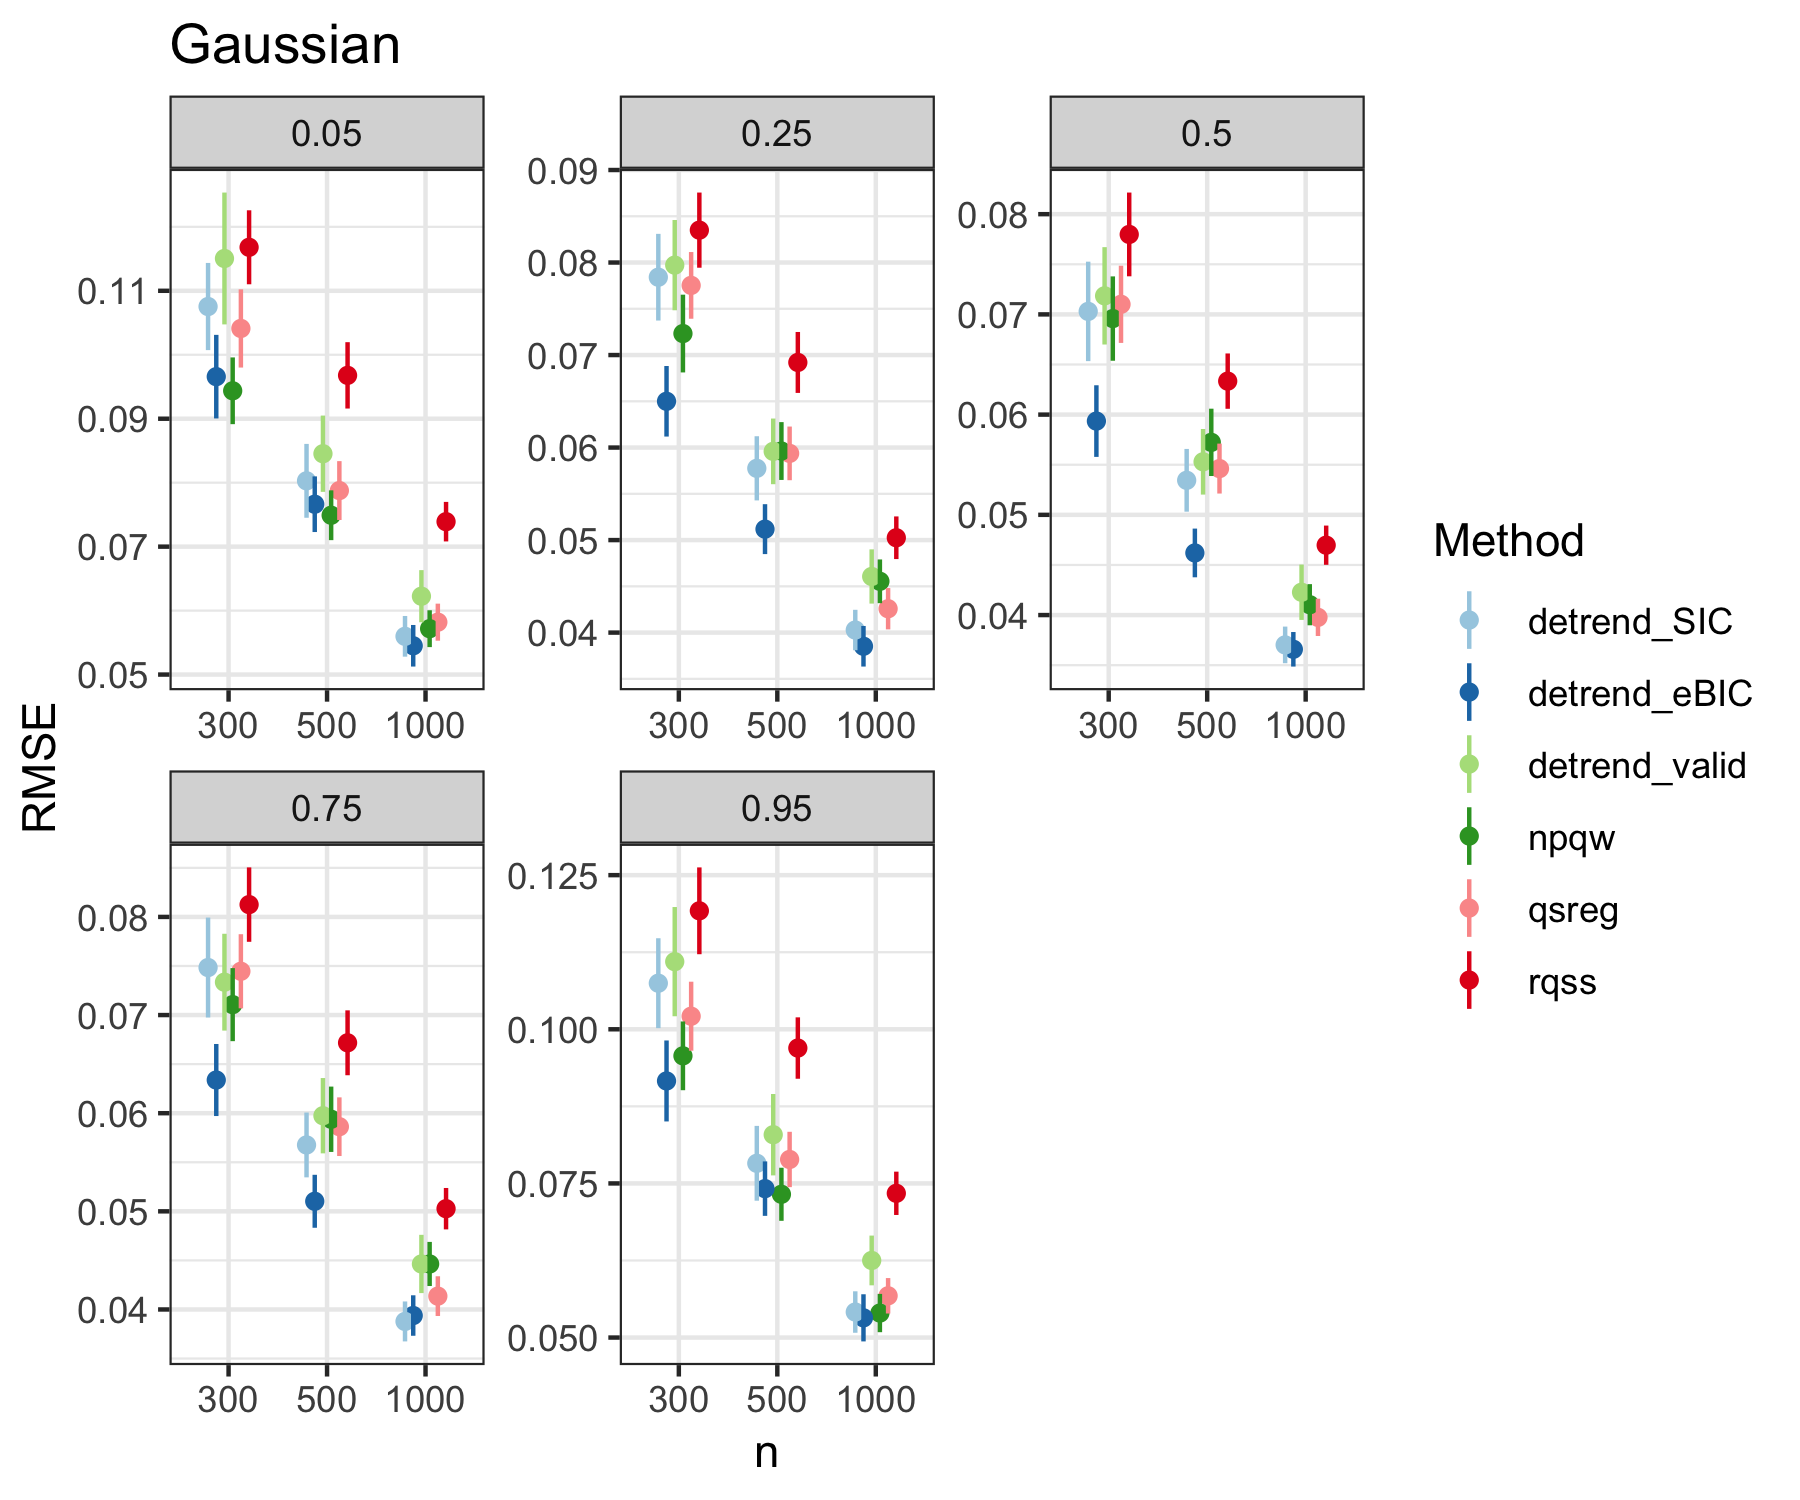
\includegraphics[width=\linewidth]{Figures/gaus_mse.png}	
	
	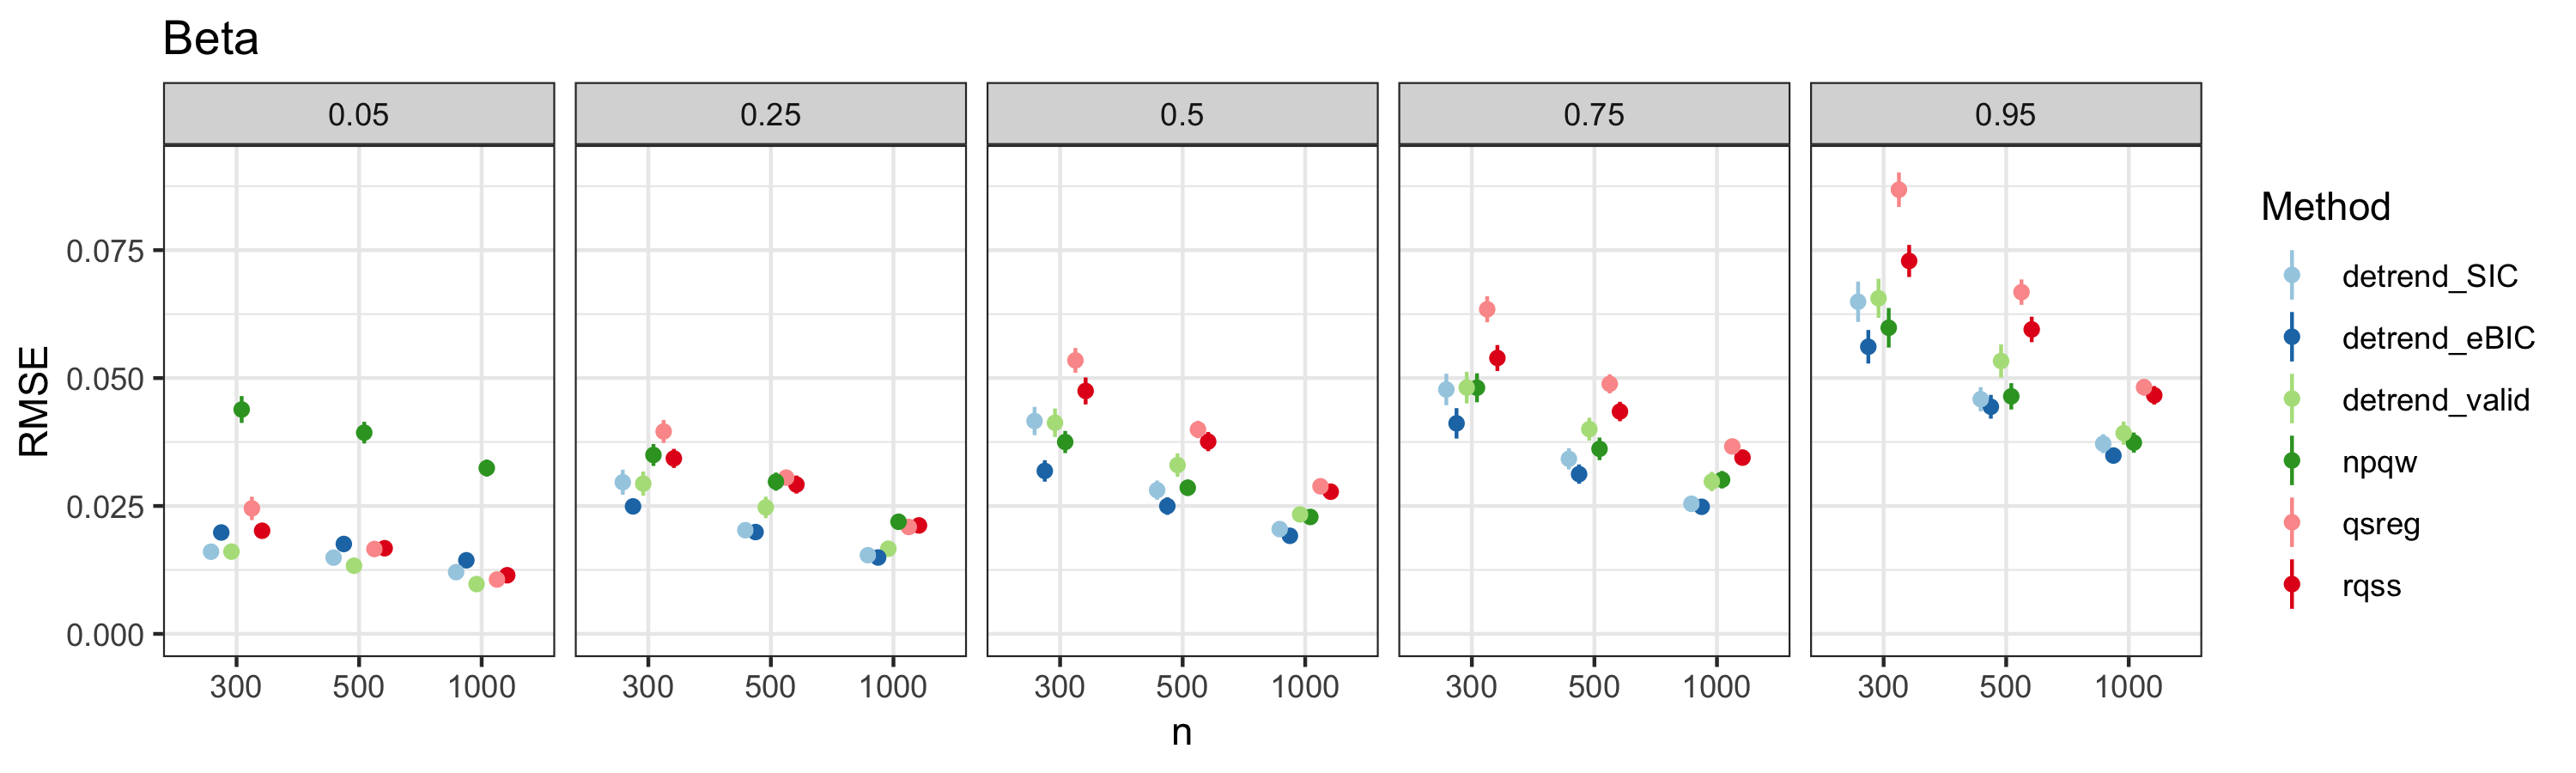
\includegraphics[width=\linewidth]{Figures/shapebeta_mse.png}
	
	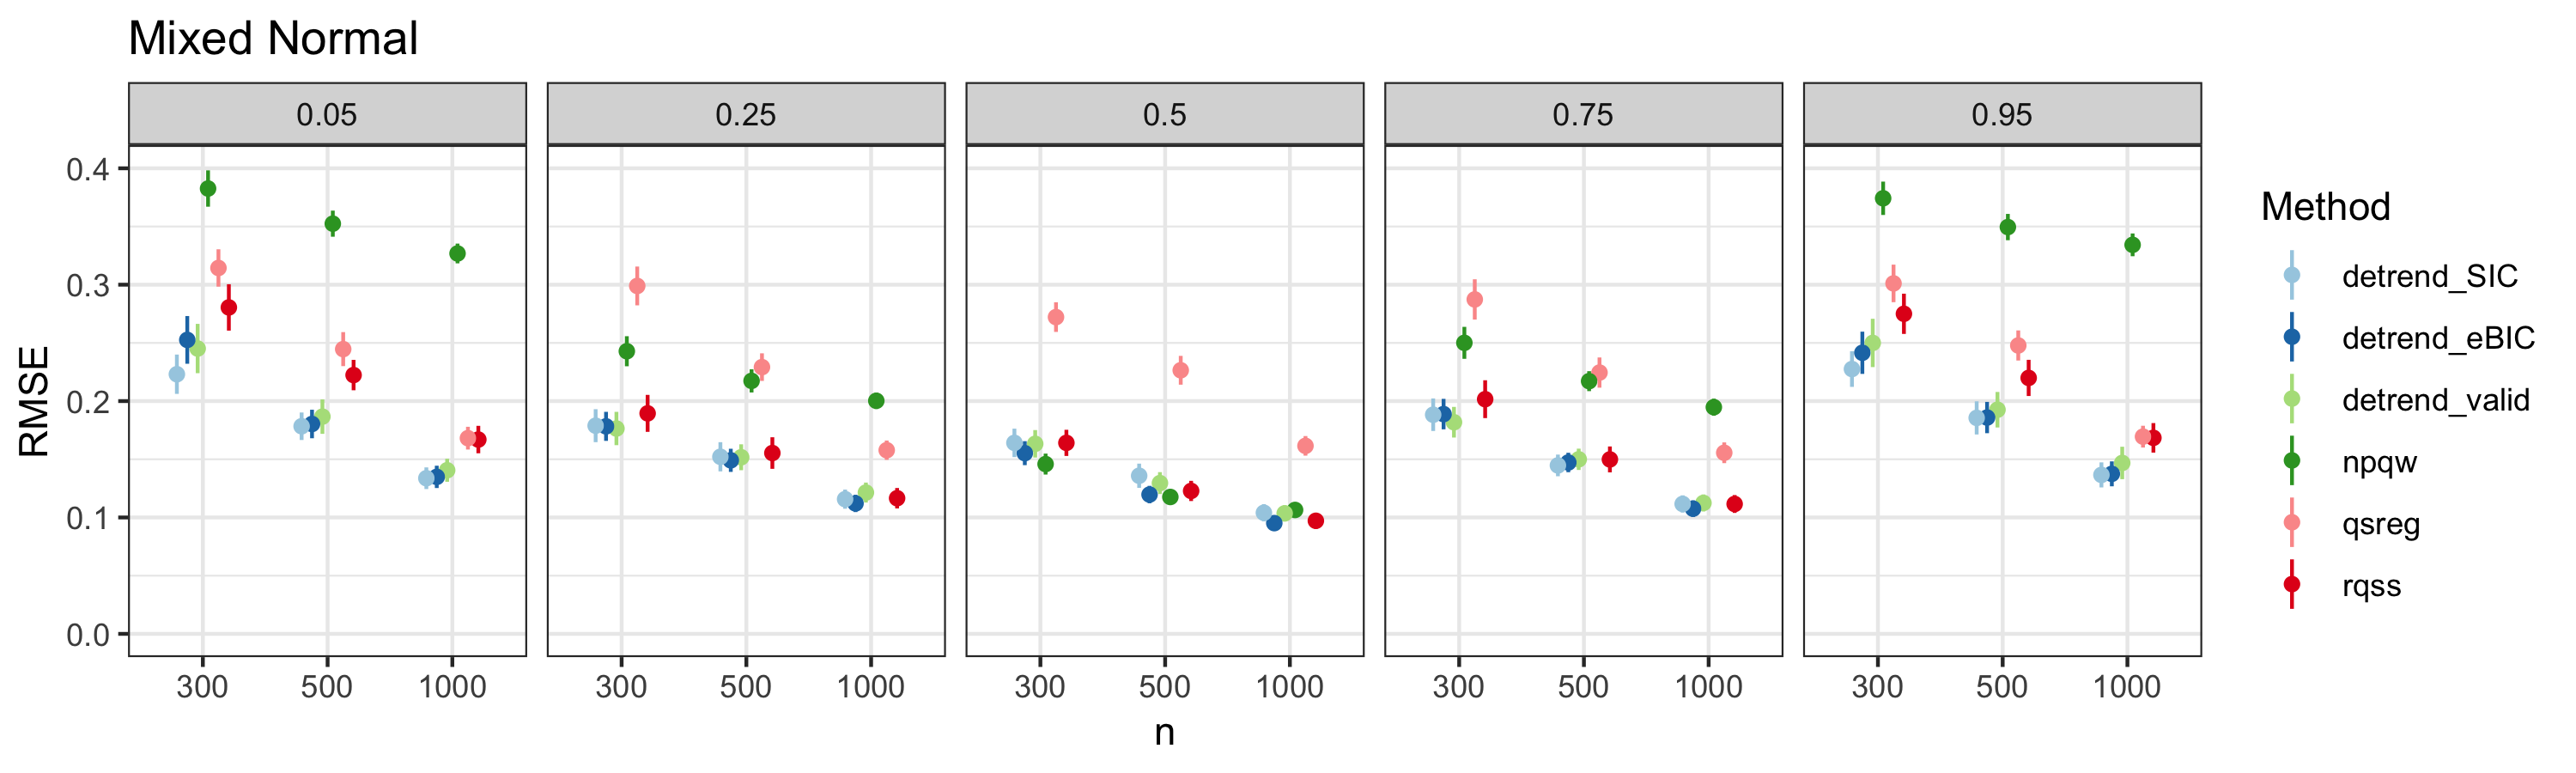
\includegraphics[width=\linewidth]{Figures/mixednorm_mse.png}
	
	In all of the designs the proposed detrend methods are either better than or comparable to existing methods. The npqw method performs particularly poorly in the mixed normal design, due to the fact that it assumes the data comes from a scale-location model which is violated in this case. 
	
	\section{Peaks Simulation}
	We use another simulation design based on the applied problem we aim to solve. We assume that the measured data can be represented by 
	\begin{equation}
	Y(t) = s(t) + b(t) + \epsilon
	\end{equation} 
	where $s(t)$ is the true signal at time $t$, $b(t)$ is the drift component that varies smoothly over time and $\epsilon \sim N(0, \sigma^2)$ is an error component. We assume $t$ is a uniformly spaced sequence between 0 and 1. We generate $b(t)$ using a cubic natural spline basis function with degrees of freedom sampled from $n/50$ to $n/25$ with equal probability, and coefficients drawn from an exponential distribution with rate 1. The true signal function is assumed to be zero with Gaussian peaks. The number of peaks is sampled from $n/100$ to $n/50$ with equal probability with centers uniformly distributed between 0.1 and 0.9 and bandwidths uniformly distributed between $1/n$ and $5/n$ and areas uniformly distributed between 0 and $20/n$. One hundred datasets were generated for $n=\{300, 500, 1000, 5000\}$. We compare the methods ability to estimate the true quantiles of $b(t) + \epsilon$  for $\tau \in \{0.01, 0.05, 0.1\}$ and calculate the RMSE. 
	
	\begin{figure}[h]
		\caption{Example of simulated peaks, baseline, and observed measurements.}
		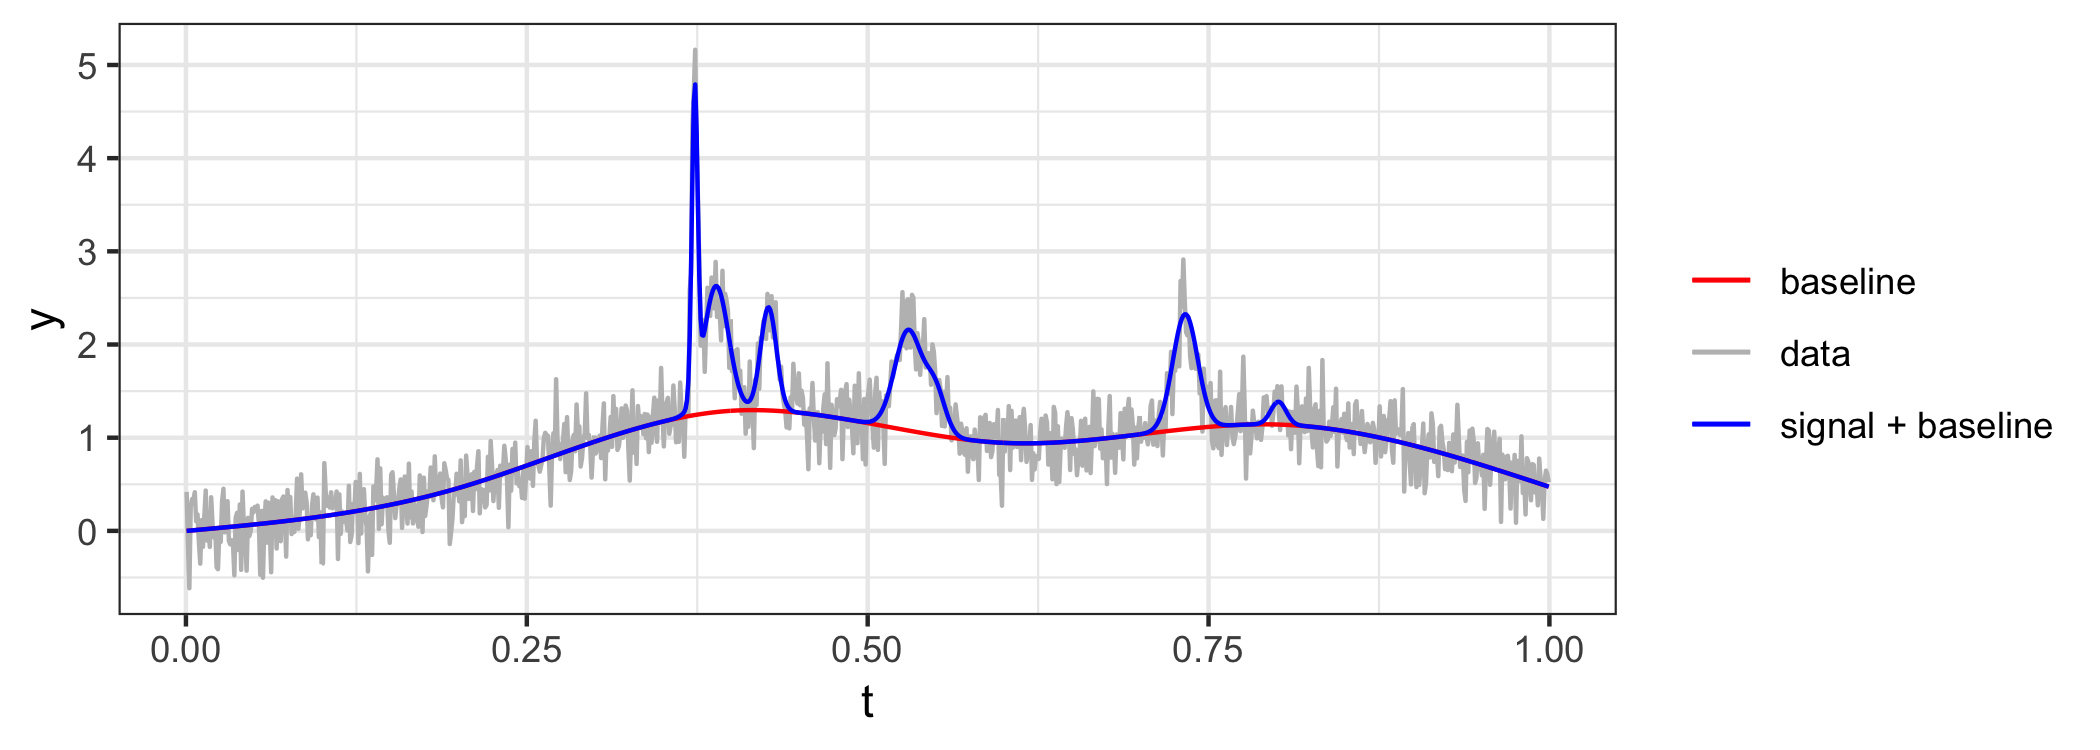
\includegraphics[width = \linewidth]{Figures/ex_peaks.png}
	\end{figure}

	In addition to the RMSE we also calculated the signal miss-classification rate. We first classified the "true" peaks function into signal or not based on a threshold of 0.1. We then classified the detrended data using three different thresholds and calculated the fraction miss-classified. An illustration of the observations classified as signal after detrending compared to the "true signal" is shown in Fig. 9. 
	
	
	\begin{figure}[h!]
		\caption{RMSEs compared to the simulated baseline function.}
		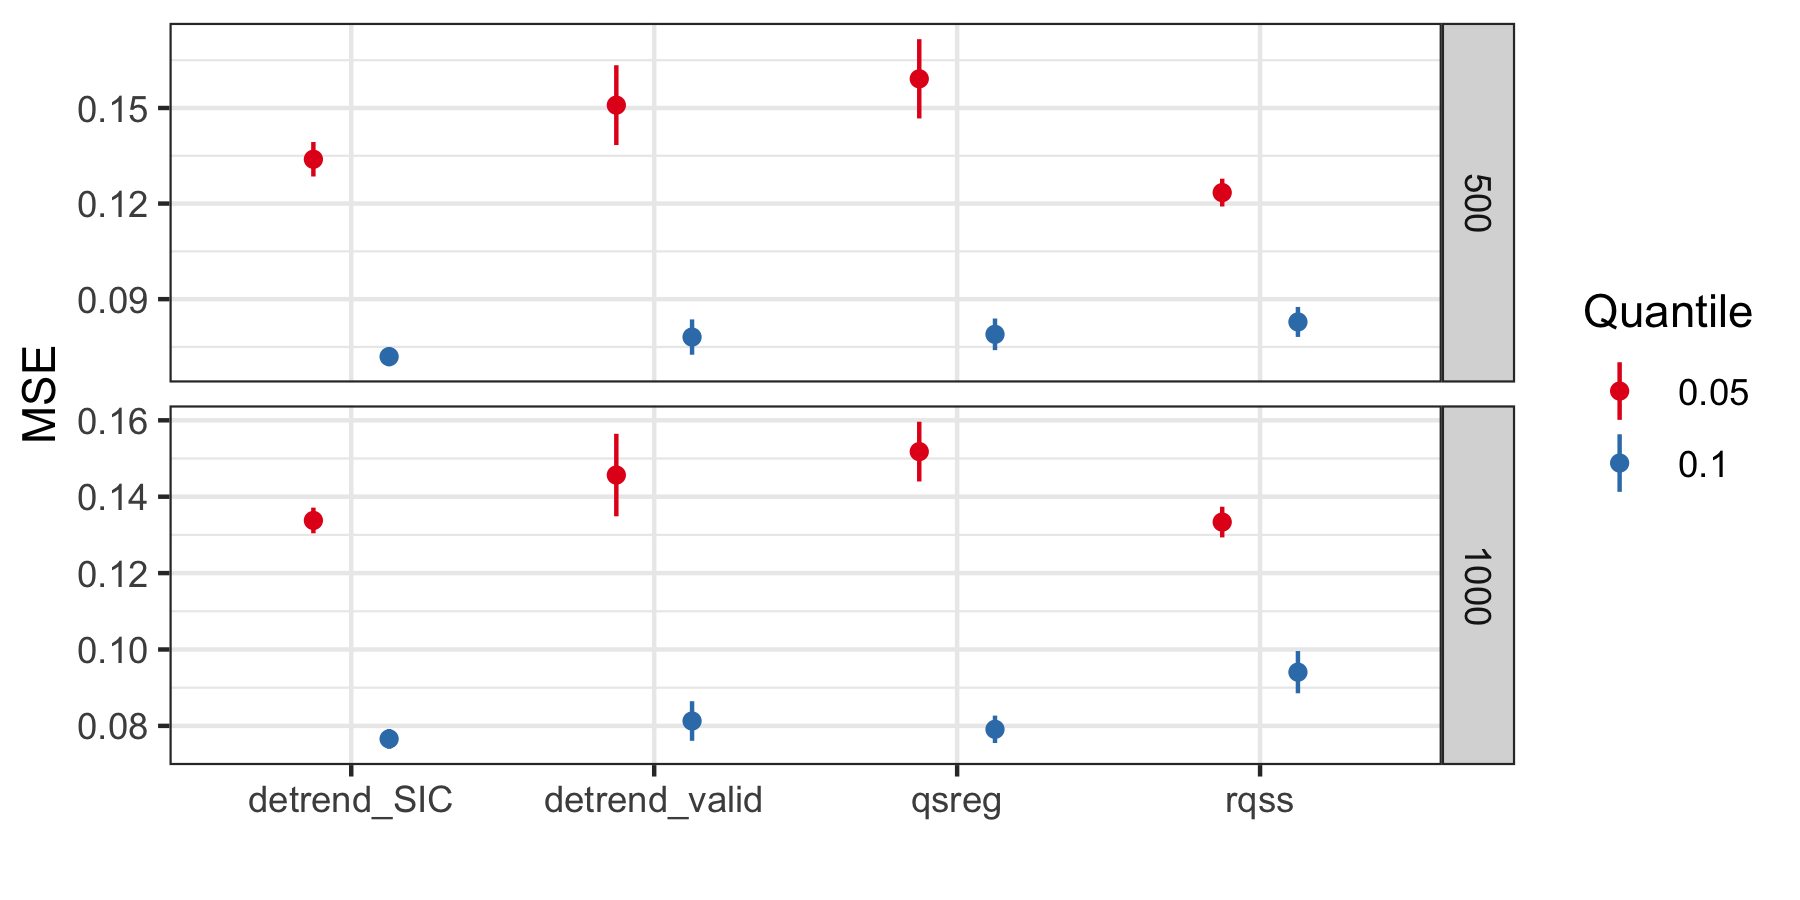
\includegraphics[width = \linewidth]{Figures/peaks_mse.png}
	\end{figure}
	
	Our detrend\_BIC method performs the best overall in terms of both RMSE and miss-classification rate. The lowest miss-classification rates were obtained using the detrend\_eBIC method and a threshold of 1 for all data sizes. While qsreg was competitive with our method in some cases, both the RMSE and miss-classification rate increased substantially with the size of the dataset. 
	
	\begin{figure}[h!]
		\caption{Example signal classification using threshold. Red indicates true signal $>0.1$, blue indicates classified as signal after baseline removal using eBIC detrendr and a threshold of 1.}
		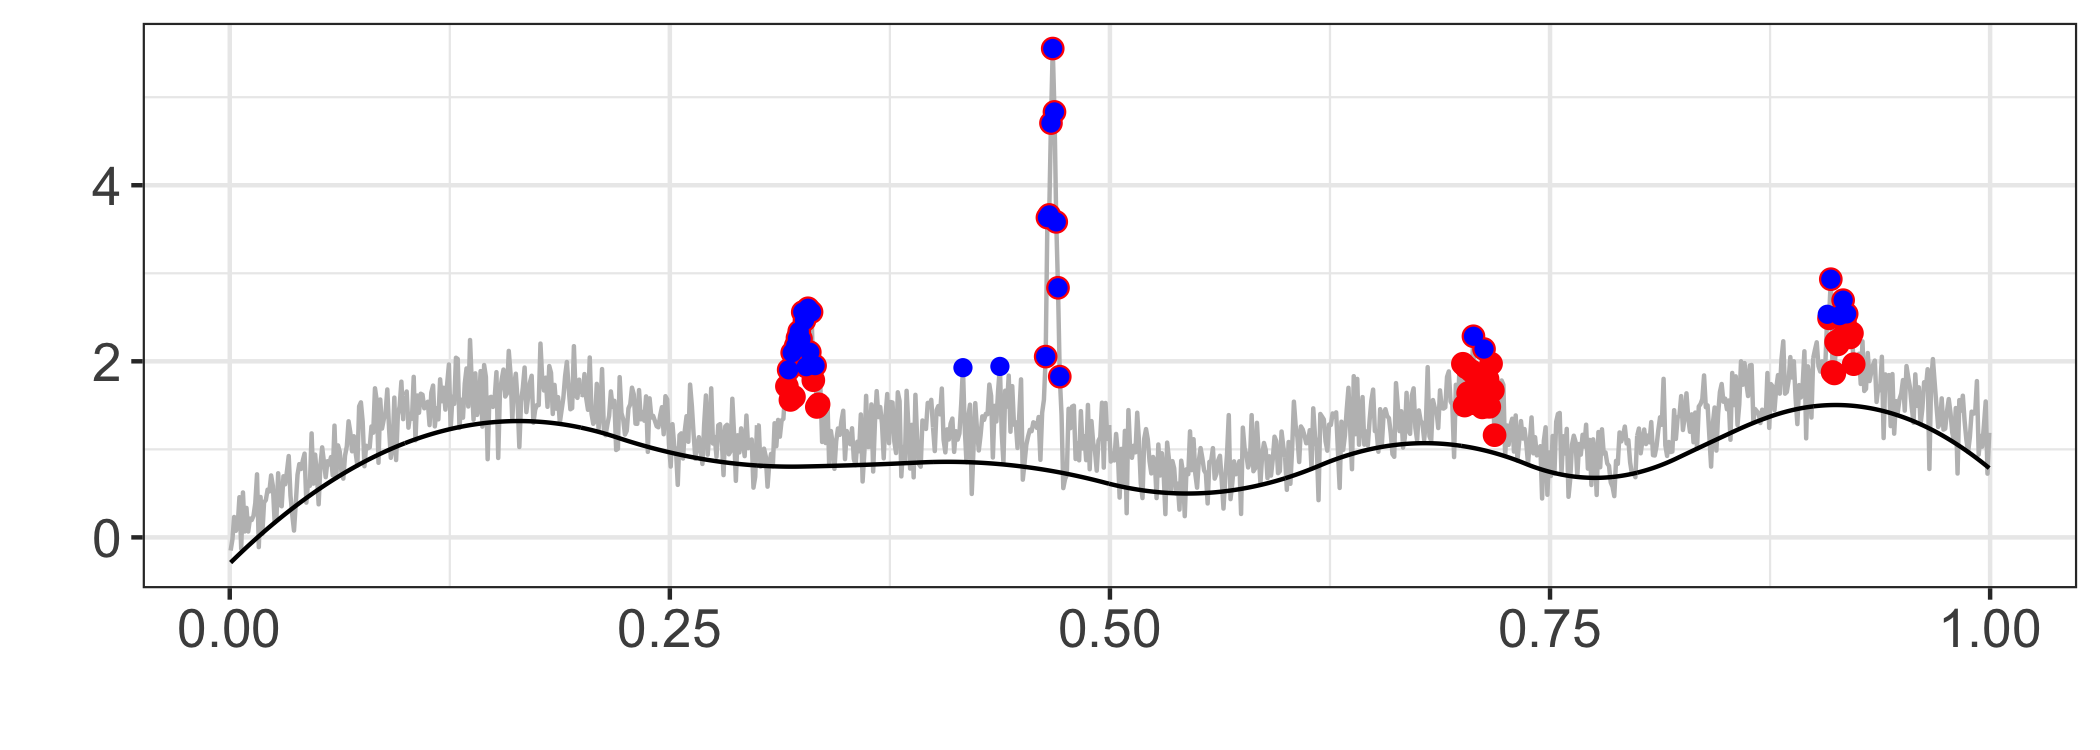
\includegraphics[width = \linewidth]{Figures/peaks_eg_class.png}
	\end{figure}
	
	\begin{figure}[h!]
		\caption{Miss-classification rates by threshold, data size, and method, values above the upper limit (npqw) not shown.}
		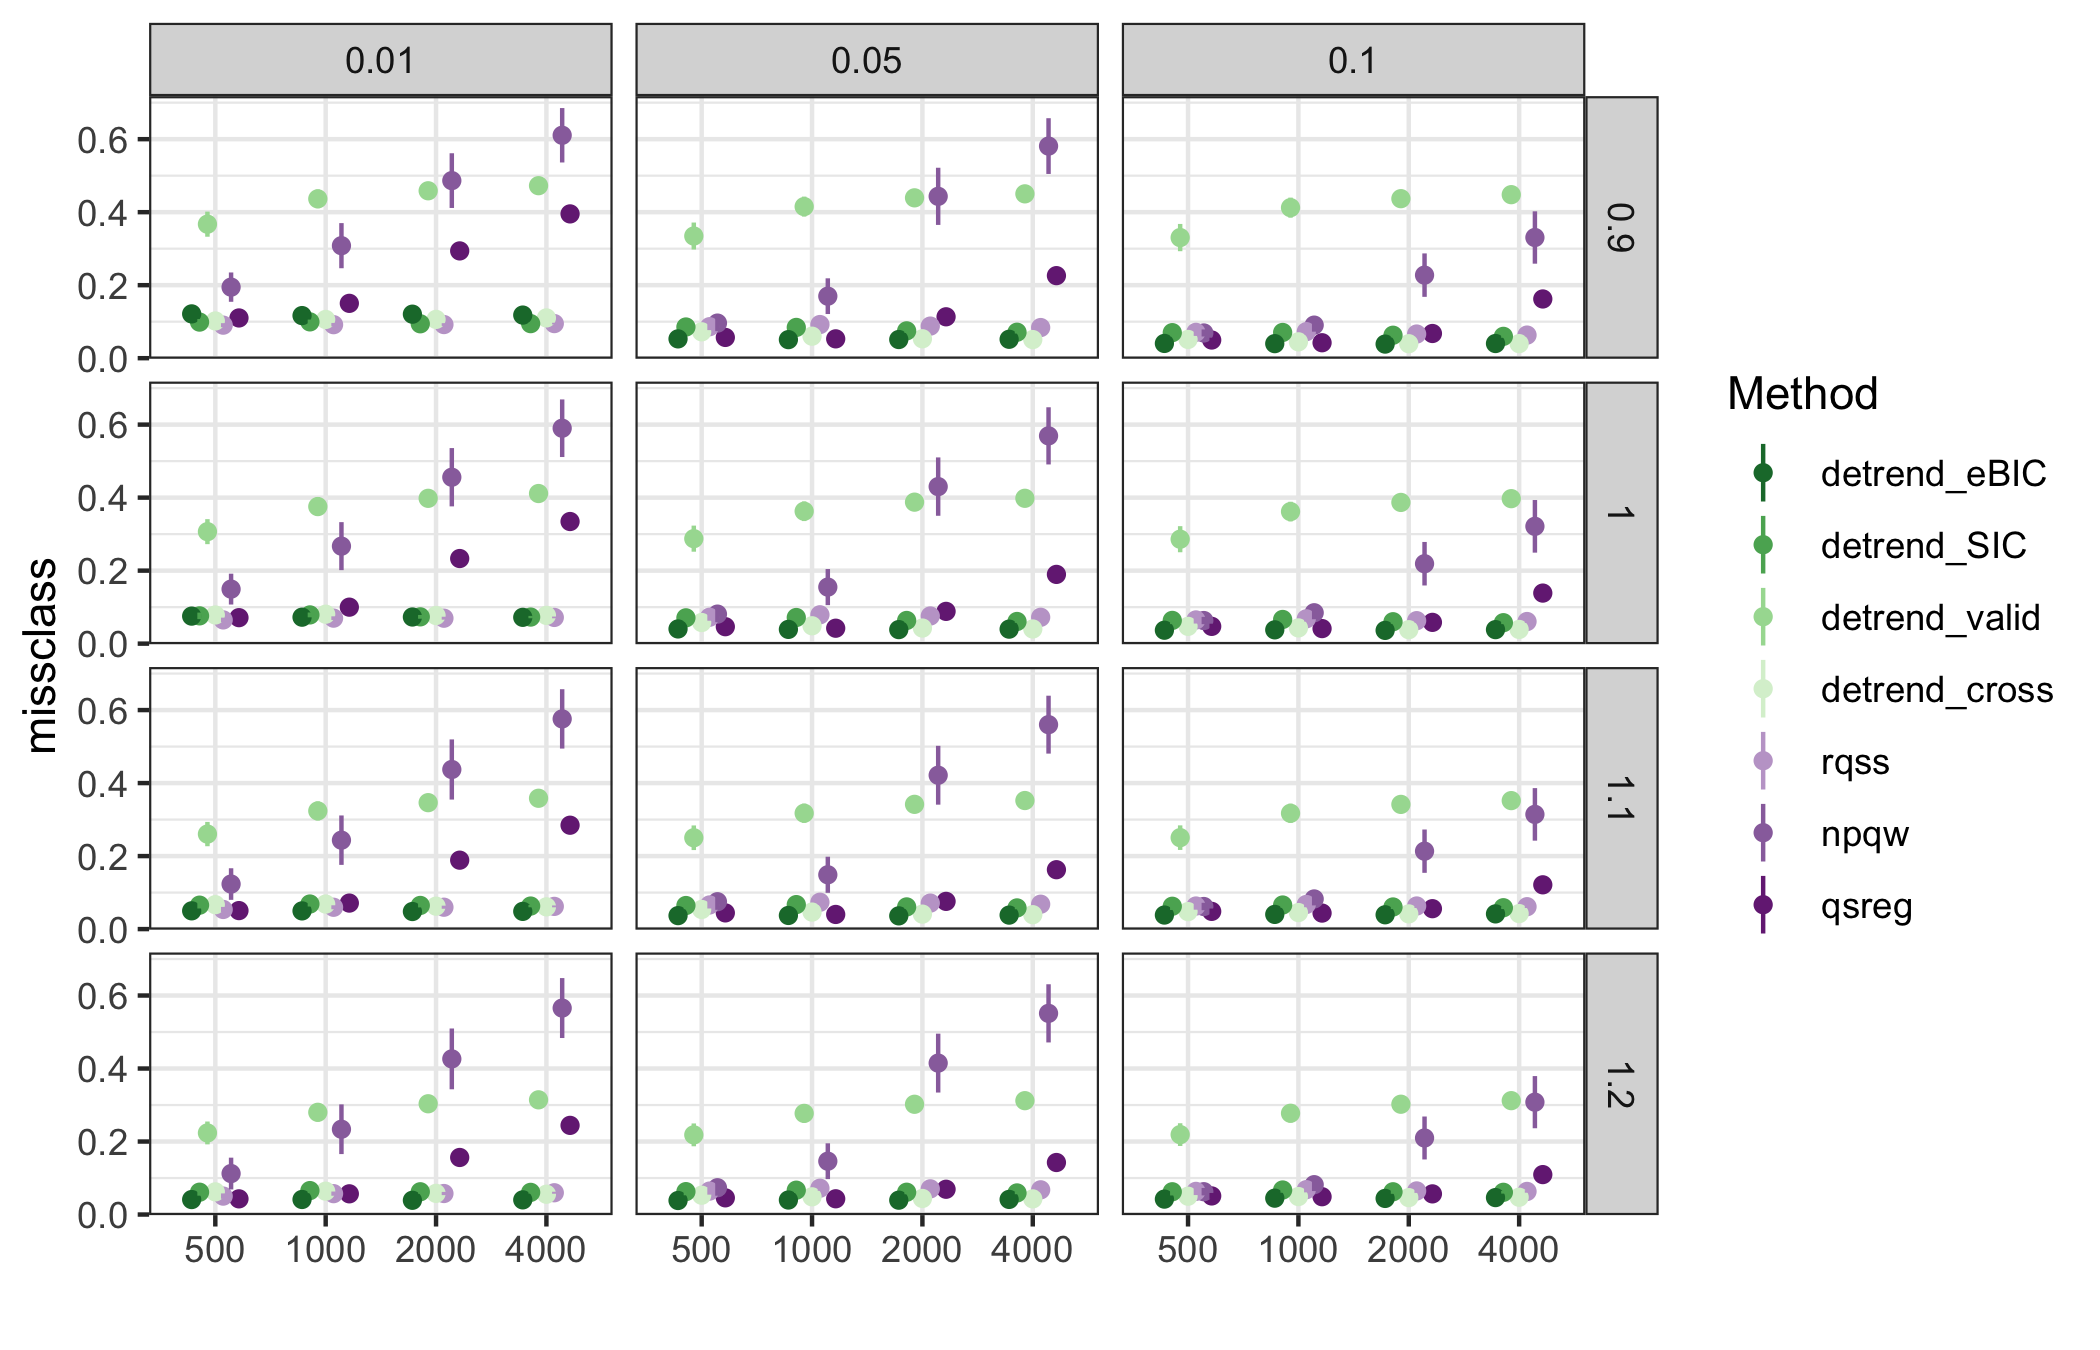
\includegraphics[width = \linewidth]{Figures/peaks_missclass.png}
	\end{figure}
	
	 
	
	\FloatBarrier
	
	\section{Application}
	
	
	Our windowed detrend method was used to removed the baseline drift from low cost air quality sensors so that the signal could be categorized using a simple threshold. The measurements were first standardized to have mean zero and variance 1. Three quantile levels for estimating the baseline trend were compared. The total dataset consisted of 52,322 observations per node. 
	The signal thresholds were set using the first 15,000 observations where it was known no signal was present. The thresholds were set as 3 times the standard deviation plus the mean of observations in this time period. The total number of seconds of signal for each node as well as the number of seconds where multiple nodes both reported signal is shown in Table 1. Table 2 shows the fraction of observations with different signal classifications by node combination. 
	
	\begin{figure}
		\caption{Low cost sensor data before drift removal (top), after drift removal using windowed detrend with eBIC (middle), 
			and zoomed in on signal area (bottom). Horizontal lines represent signal thresholds.}
		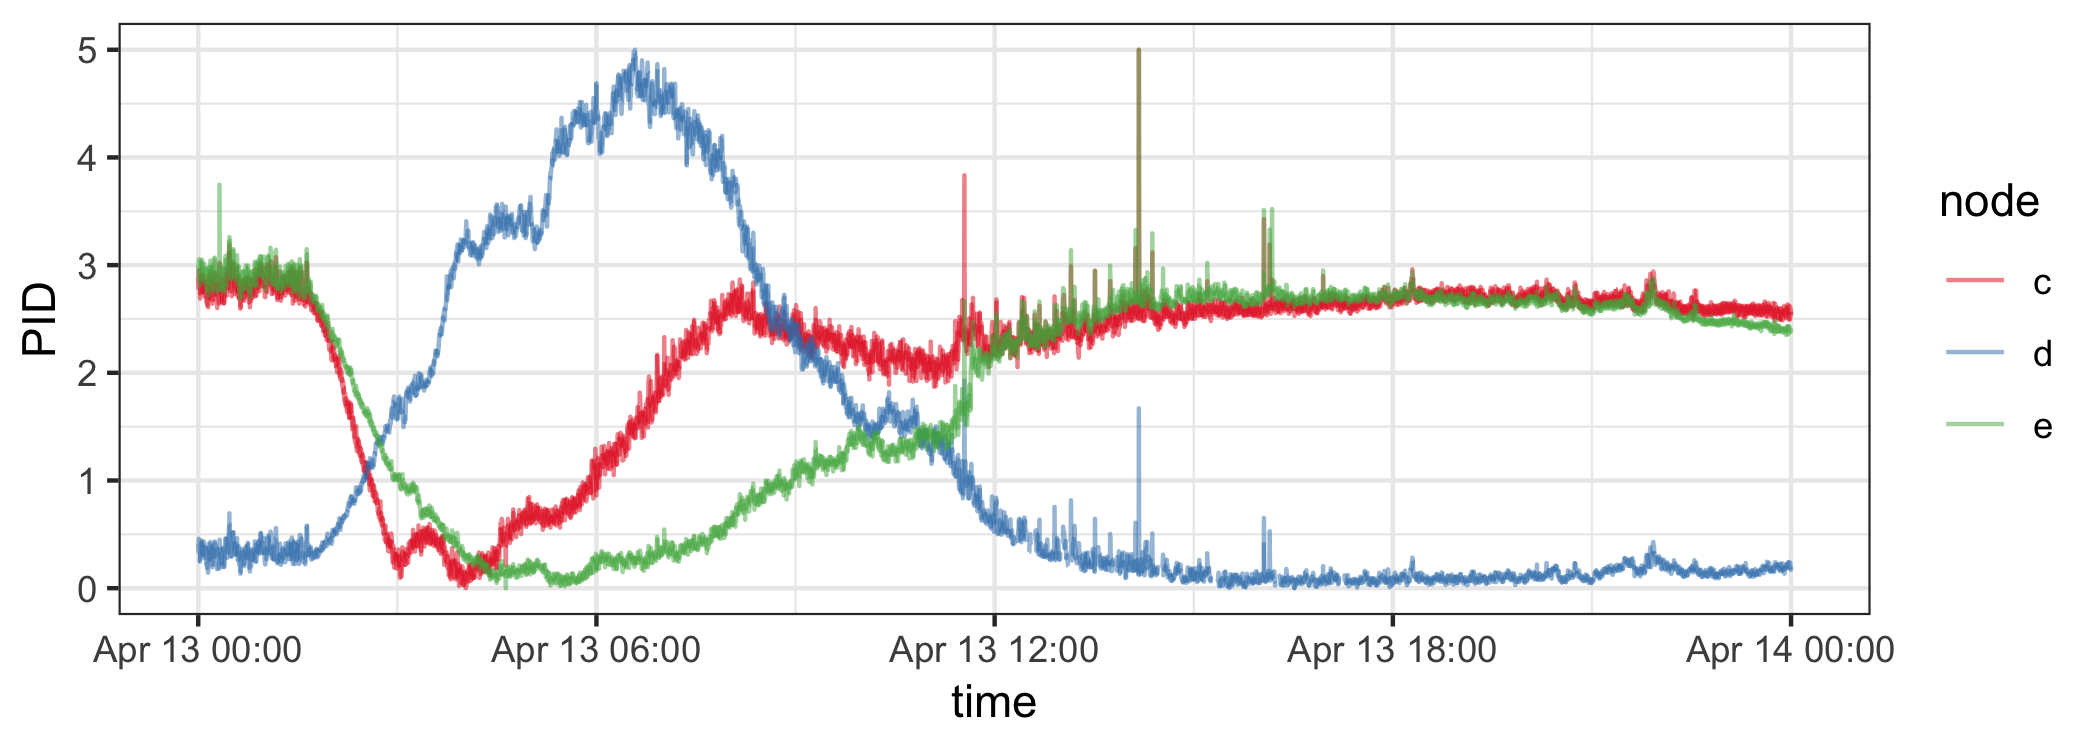
\includegraphics[width = \linewidth]{Figures/uncorrected_data.png}
		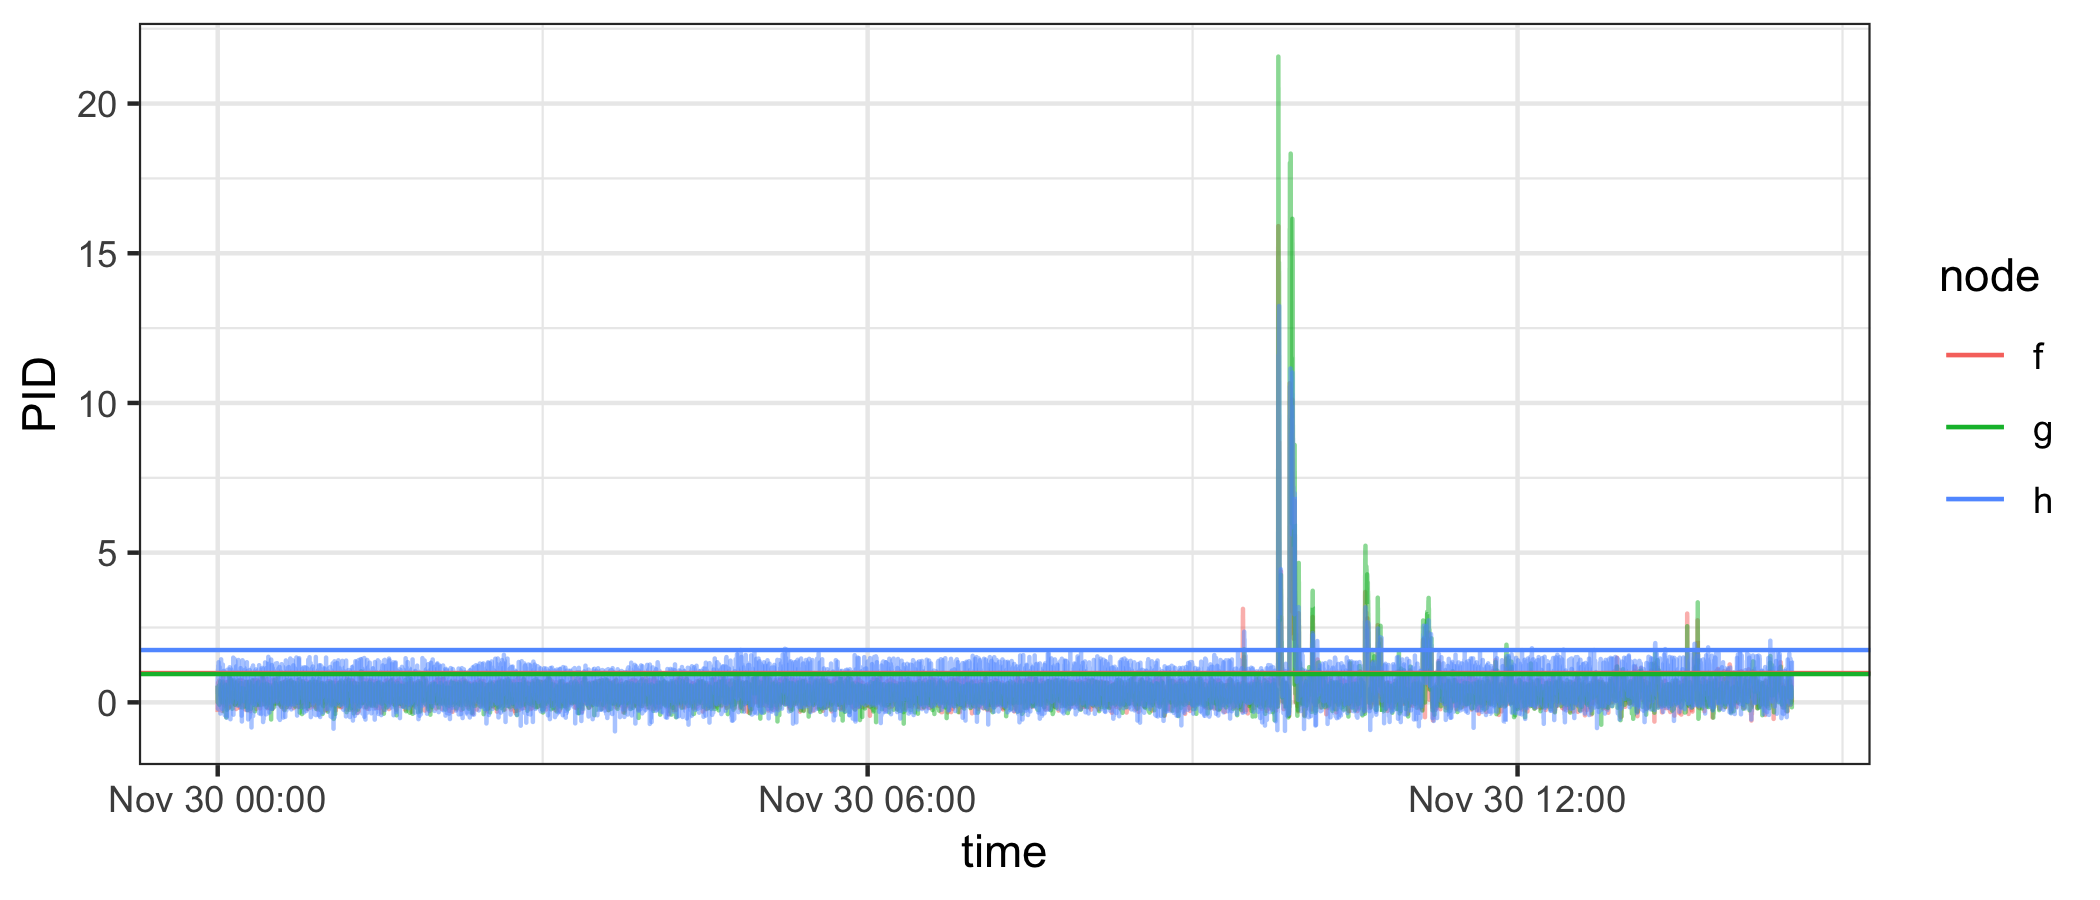
\includegraphics[width = \linewidth]{Figures/corrected_data.png}
		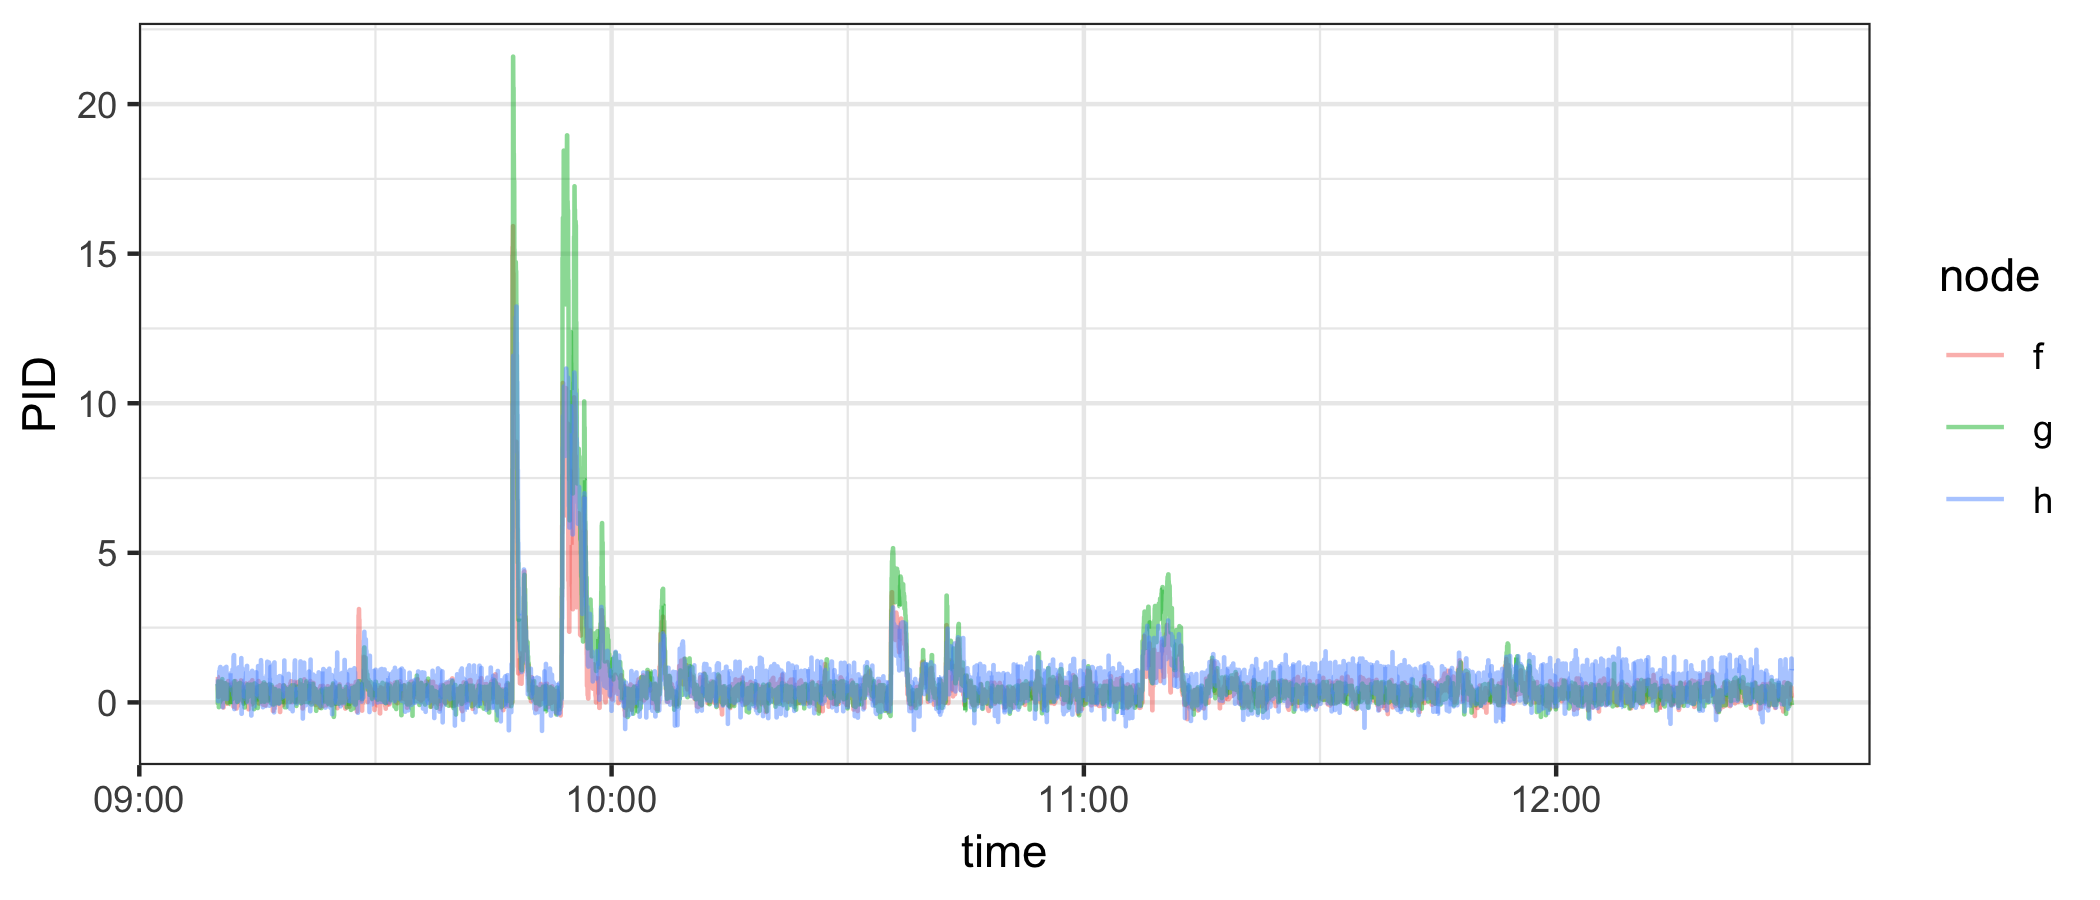
\includegraphics[width = \linewidth]{Figures/corrected_zoom_data.png}
	\end{figure}

	%latex.default(miss_df, rowname = "", title = "", file = sprintf("../Manuscript/application_missclass.tex"),     caption = "Fraction of seconds with different signal (0/1) classifications.")%
\begin{table}[!tbp]
\caption{Fraction of seconds with different signal (0/1) classifications.\label{}} 
\begin{center}
\begin{tabular}{llrrr}
\hline\hline
\multicolumn{1}{l}{}&\multicolumn{1}{c}{Comparison}&\multicolumn{1}{c}{tau 0.1}&\multicolumn{1}{c}{tau 0.2}&\multicolumn{1}{c}{tau 0.3}\tabularnewline
\hline
&fg&$0.018$&$0.016$&$0.015$\tabularnewline
&fh&$0.015$&$0.013$&$0.011$\tabularnewline
&gh&$0.018$&$0.018$&$0.017$\tabularnewline
\hline
\end{tabular}\end{center}
\end{table}
	
	%latex.default(bind_rows(signal_ct, signal_comb), rowname = "",     title = "", file = sprintf("../Manuscript/application_signal.tex"),     caption = "Seconds of signal by node combination and quantile level.")%
\begin{table}[!tbp]
\caption{Seconds of signal by node combination and quantile level.\label{}} 
\begin{center}
\begin{tabular}{llrrr}
\hline\hline
\multicolumn{1}{l}{}&\multicolumn{1}{c}{Node}&\multicolumn{1}{c}{tau 0.1}&\multicolumn{1}{c}{tau 0.2}&\multicolumn{1}{c}{tau 0.3}\tabularnewline
\hline
&f&$1219$&$1079$&$ 933$\tabularnewline
&g&$1500$&$1410$&$1363$\tabularnewline
&h&$ 703$&$ 594$&$ 605$\tabularnewline
&fh&$ 561$&$ 491$&$ 487$\tabularnewline
&gh&$ 621$&$ 529$&$ 540$\tabularnewline
&fg&$ 891$&$ 832$&$ 764$\tabularnewline
&fgh&$ 542$&$ 469$&$ 469$\tabularnewline
\hline
\end{tabular}\end{center}
\end{table}

	
	
	\section{Conclusion}
	\label{sec:conc}
	
	
	\bigskip
	\begin{center}
		{\large\bf SUPPLEMENTARY MATERIAL}
	\end{center}
	
	\begin{description}
		
		\item[R-package for detrend routine:] R-package detrendr containing code to perform the diagnostic methods described in the article. The package also contains all datasets used as examples in the article. (GNU zipped tar file)
				
	\end{description}
	
	\section{References}

	
	\bibliographystyle{asa}
	\bibliography{detrendify}
	
\end{document}

